\chapter{Building a best choice recommendation}
\label{sec:4}

\abstract*{  This chapter presents the \Rubis best choice recommender system. Our approach is illustrated with building a best office site recommendation. We show how to explore the given performance tableau and compute the corresponding outranking digraph. After presenting the pragmatic principles that govern our best choice recommendation algorithm we solve the best office-location choice problem.}

\begin{quotation}
  ``... \emph{The goal of our research was to design a resolution method} ... \emph{that is easy to put into practice, that requires as few and reliable hypotheses as possible, and that meets the needs} [of the decision maker]...''

  --\citep*{ROY-1966}\index{Roy@\textsl{B. Roy}}.
\end{quotation}
\vspace{1cm}

\abstract{ This chapter presents the \Rubis best choice recommender system. Our approach is illustrated with a best office location selection problem. We show how to explore the given performance tableau and compute the corresponding outranking digraph. After presenting the pragmatic principles that govern our best choice recommendation algorithm we solve the best office location choice problem.}

\section{What office-location to choose?}
\label{sec:4.1}

A SME, specialised in printing and copy services, has to move into new offices, and its CEO has gathered seven \emph{potential new office locations} (see Tab.~\vref{tab:4.1}).
\begin{table}[ht]
\caption{The potential new office locations}
\label{tab:4.1}       % Give a unique label
\begin{center}
  %\begin{small}
    \begin{tabular}{c|l|l|l}
      \svhline\noalign{\smallskip}
      ID & Name & Address & Comment\\
      \noalign{\smallskip}\hline\noalign{\smallskip}
    A &   Ave  &  Avenue de la liberté &  High standing city center\\
    B &   Bon  &  Bonnevoie &             Industrial environment\\
    C &   Ces  &  Cessange &              Residential suburb location\\
    D &   Dom  &  Dommeldange &           Industrial suburb environment\\
    E &   Bel  &  Esch-Belval &           New and ambitious urbanisation far from the city\\
    F &   Fen  &  Fentange &              Out in the countryside\\
      G &   Gar  &  Avenue de la Gare &     Main city shopping street\\
      \noalign{\smallskip}\hline
    \end{tabular}
  %\end{small}
\end{center}
\end{table}

Three \emph{decision objectives}, in order of decreasing importance, are guiding the CEO's choice:
\begin{enumerate}[leftmargin=1cm]
\item \emph{maximise} the future turnover of the SME,
\item \emph{minimise} the future yearly costs induced by the moving,
\item \emph{maximise} the new working conditions.
\end{enumerate}

The decision consequences to take into account for evaluating the potential new office locations with respect to each one of the three objectives are modelled by the \emph{family of performance criteria} \footnote{See \citealp{ROY-2000}} shown in Table~\vref{tab:4.2} below.
\begin{table}[ht]
\caption{The family of performance criteria}
\label{tab:4.2}       % Give a unique label
\begin{center}
    \begin{tabular}{l|c|c|c|l}
      \svhline\noalign{\smallskip}
      Objective & ID & Name & Weight & Comment\\
      \noalign{\smallskip}\hline\noalign{\smallskip}
    Yearly costs  &       Ct &   Costs &  45 &     Annual rent, charges, and cleaning\\
    \             &  \      & \        &  \ & \ \\
    Future turnover   &   Pr  & Proximity  & 32 & Distance from town center\\
    Future turnover   &   V  &  Visibility & 26 & Circulation of potential customers \\
    Future turnover   &   St &   Standing & 23 &   Image and presentation\\
    \                 &   \   & \          &  \ & \  \\
    Working conditions &  W  &  Space   &   10 &  Working space\\
    Working conditions &  Cf &  Comfort  &  6 &  Quality of office equipment\\
    Working conditions &  P  &  Parking  &  3 &  Available parking facilities\\
      \noalign{\smallskip}\hline
    \end{tabular}   
  \end{center}
\end{table}

In Table~\vref{tab:4.2} we notice that the \emph{Costs} criterion admits the highest significance weight ($45$), followed by the \emph{Future turnover} criteria $(32, 26, 23)$, The \emph{Working conditions} criteria are the less significant $(10, 6, 3)$ \footnote{These criteria weights were supposedly established with a swing weighing MCDA method \citep{KEE-1976}.}. It follows that the CEO considers \emph{maximising the future turnover} the most important objective ($(32 + 26+ 23) = 81$), followed by minimising the future yearly costs ($45$), and less important, \emph{maximising working conditions} ($(10 + 6 + 3) = 19$). 

The evaluations of the seven potential new locations on each performance criterion are gathered in a \emph{performance table} shown in Table~\vref{tab:4.3}.
\begin{table}[ht]
\caption{Performance evaluations of the potential office locations}
\label{tab:4.3}       % Give a unique label
\begin{center}
    \begin{tabular}{l|c|c|c|c|c|c|c}
      \svhline\noalign{\smallskip}
    Criterion  &    A  &      B &       C &       D &       E &        F &        G\\
       \noalign{\smallskip}\hline\noalign{\smallskip}

    Costs      &   35.0K€ &  17.8K€  & 6.7K€  &  14.1K€ &  34.8K€ &  18.6K€ &  12.0K€\\
    \          &   \      &  \     &   \     &   \    &    \    &    \    &    \ \\
    Proximity     &   100    &  20 &      80    &   70    &   40    &   0    &    60 \\
    Visibility     &   60     &  80  &     70    &   50    &   60    &   0    &    100 \\
    Standing      &   100   &   10   &    0     &   30    &   90    &   70   &    20 \\
    \           &   \     &   \    &    \     &   \     &   \     &   \    &    \  \\
    Working space      &   75    &   30   &    0     &   55    &   100   &   0    &    50  \\
    Working comfort      &   0     &   100  &    10    &   30    &   60    &   80   &    50 \\
    Parking     &   90    &   30   &    100   &   90    &   70    &   0    &    80 \\
      \noalign{\smallskip}\hline
    \end{tabular}
  \end{center}
\end{table}
All criteria, except the \emph{Costs} Criterion, admit for evaluation a qualitative satisfaction scale from $0\%$ (weakest) to $100\%$ (highest). One may thus notice that location \texttt{A} (\emph{Ave}) is the most expensive, but also $100\%$ satisfying the \emph{Proximity} as well as the  \emph{Standing} criterion. Whereas location \texttt{C} (\emph{Ces}) is the cheapest one; providing however no satisfaction at all on both the \emph{Standing} and the \emph{Working Space} criteria.

Concerning yearly costs, we suppose that the CEO is indifferent up to a performance difference of $1000.00$€, and he actually prefers a location when there is at least a positive difference of $2500.00$€. The evaluations observed on the six qualitative criteria (measured in percentages of satisfaction) are very subjective and rather imprecise. The CEO is hence \emph{indifferent} up to a satisfaction difference of $10\%$, and he claims a significant \emph{preference} when the satisfaction difference is at least of $20\%$.  Furthermore, a satisfaction difference of $80\%$ represents for him a \emph{considerably large} performance difference, triggering the case given a \emph{polarisation} of the preferential situation \citep{BIS-2013}. 

In view of Table~\vref{tab:4.3}, what is now the office location we may recommend to the CEO as \textbf{best choice}?

\section{The given performance tableau}
\label{sec:4.2}


The file \texttt{officeChoice.py}, stored in the \texttt{examples} directory of the \Digraph resources, provides a corresponding \texttt{PerformanceTableau}\index{PerformanceTableau@\texttt{PerformanceTableau} class} object. We can inspect its actual content with the computing resources provided by the \texttt{perfTabs} module \index{perfTabs@\texttt{perfTabs} module}.
\begin{lstlisting}[caption={Inspecting the \texttt{officeChoice} performance tableau.},label=list:4.1]
>>> from perfTabs import PerformanceTableau
>>> pt = PerformanceTableau('officeChoice')
>>> pt
 *------- PerformanceTableau instance description ------*
   Instance class     : PerformanceTableau
   Instance name      : officeChoice
   Actions            : 7
   Objectives         : 3
   Criteria           : 7
   NaN proportion (%) : 0.0
   Attributes         : ['name', 'actions', 'objectives',
                         'criteria', 'weightPreorder',
			 'NA', 'evaluation']
>>> pt.showPerformanceTableau()
 *----  performance tableau -----*
  Criteria|  'Ct'       'Cf'   'P'   'Pr'   'St'    'V'    'W'   
  Weights |  45.00      6.00   3.00  32.00  23.00  26.00  10.00    
  --------|----------------------------------------------------
   'Ave'  | -35000.00   0.00  90.00 100.00 100.00  60.00  75.00  
   'Bon'  | -17800.00 100.00  30.00  20.00  10.00  80.00  30.00  
   'Ces'  |  -6700.00  10.00 100.00  80.00   0.00  70.00   0.00  
   'Dom'  | -14100.00  30.00  90.00  70.00  30.00  50.00  55.00  
   'Bel'  | -34800.00  60.00  70.00  40.00  90.00  60.00 100.00  
   'Fen'  | -18600.00  80.00   0.00   0.00  70.00   0.00   0.00  
   'Gar'  | -12000.00  50.00  80.00  60.00  20.00 100.00  50.00  
\end{lstlisting}

We thus recover all the input data shown in Section~\ref{sec:4.1}. Notice that the \emph{negative} evaluations of the \emph{Costs} criterion indicate a negative preference direction: the \emph{lower} the costs, the \emph{better} it is.

The \texttt{showCriteria()}\index{showCriteria@\texttt{showCriteria()}} method evaluates the actual preference discrimination we observe on each performance criterion.
\begin{lstlisting}[caption={Inspecting the performance criteria.},label=list:4.2]
>>> pt.showCriteria(IntegerWeights=True)
 *----  criteria -----*
  Ct 'Costs'
   Preference direction: min
   Scale = (0.00, 50000.00)
   Weight = 45
   Threshold ind : 1000.00 + 0.00x ;  percentile:  9.52 §\label{line:4.2.7}§
   Threshold pref : 2500.00 + 0.00x ; percentile: 14.29 §\label{line:4.2.8}§
  Cf 'Comfort'
   Preference direction: max
   Scale = (0.00, 100.00)
   Weight = 6
   Threshold ind : 10.00 + 0.00x ;  percentile:   9.52 §\label{line:4.2.13}§
   Threshold pref : 20.00 + 0.00x ; percentile:  28.57 §\label{line:4.2.14}§
   Threshold veto : 80.00 + 0.00x ; percentile:  90.48 §\label{line:4.2.15}§
   ...
   ...
\end{lstlisting}

On the \emph{Costs} criterion, $9.5\%$ of the performance differences are considered insignificant and $14.3\%$ below the preference discrimination threshold (see Lines~\ref{line:4.2.7}-\ref{line:4.2.8} in List.~\vref{list:4.2}). On the qualitative \emph{Comfort} criterion, we observe again $9.5\%$ of insignificant performance differences (line~\ref{line:4.2.13}). Due to the imprecision in the subjective evaluations, we notice here $28.6\%$ of performance differences below the preference discrimination threshold (Line~\ref{line:4.2.14}). Furthermore, $100.0 - 90.5 = 9.5\%$ of the performance differences are judged \emph{considerably large} (Line~\ref{line:4.2.15}) and will trigger hence a polarisation of the concerned outranking situations \citep{BIS-2013}. Same information is available for all the other criteria. 
 
A colourful comparison of all the evaluations is shown in Figure~\vref{fig:4.1} by the \emph{heatmap}\index{showHTMLPerformanceHeatmap@\texttt{showHTMLPerformanceHeatmap()}} statistics, illustrating the respective quantile class of each evaluation. As the set of potential alternatives is tiny, we choose here a classification into performance quintiles.
\begin{lstlisting}
>>> pt.showHTMLPerformanceHeatmap(colorLevels=5,\
...                              rankingRule=None)
\end{lstlisting}
    \begin{figure}[ht]
%\sidecaption
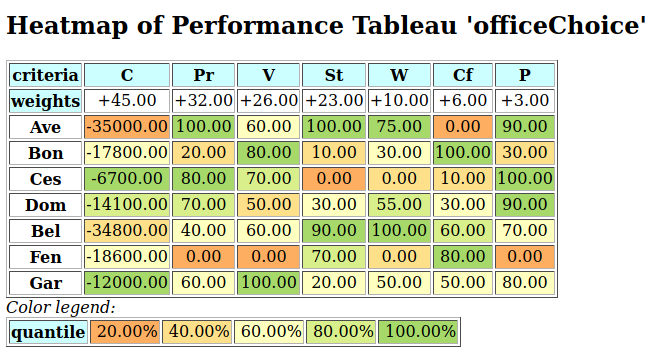
\includegraphics[width=0.8\hsize]{Figures/4-1-officeChoiceHeatmap.png}
\caption{Unranked heatmap of the office choice performance tableau}
\label{fig:4.1}       % Give a unique label
\end{figure}

Location \texttt{Ave} shows extreme and contradictory evaluations: highest \emph{Costs} and no \emph{Working Comfort} on the one hand, and total satisfaction with respect to \emph{Standing}, \emph{Proximity} and \emph{Parking facilities} on the other hand. Similar, but opposite, situation is given for location \texttt{Ces}: unsatisfactory \emph{Working Space}, no \emph{Standing} and no \emph{Working Comfort} on the one hand, and lowest \emph{Costs}, best \emph{Proximity} and \emph{Parking facilities} on the other hand. Contrary to these contradictory alternatives, we observe two appealing compromise alternatives: locations \texttt{Dom} and \texttt{Gar}. Finally, location \texttt{Fen} is clearly the less satisfactory alternative of all.

To help now the CEO choosing the best office location, we are going to compute pairwise outranking situations on the set of potential decision alternatives (see \citealp{BIS-2013}).

\section{Computing the outranking digraph}
\label{sec:4.3}

\begin{definition}[Outranking situation]\label{def:outranking}\index{outranking!situation}

\noindent For two potential decision alternatives $x$ and $y$:
\begin{itemize}[leftmargin=0.5cm,rightmargin=0.5cm]
\item ``Alternative $x$ \emph{outranks} alternative $y$'', denoted $(x \succsim y)$, is given when:
   \begin{enumerate}[nosep]
     \item A \emph{majority} of criteria significance warrants that alternative $x$ is \emph{at least as well evaluated as} alternative $y$, and
     \item \emph{No considerable} negative performance difference is observed on any criterion.      
    \end{enumerate}
\item ``Alternative $x$ \emph{does not outrank} $y$'', denoted $(x \not\succsim y)$, is given when:
   \begin{enumerate}[nosep]
    \item Only a \emph{minority} of criteria significance warrants that alternative $x$ is \emph{at least as well evaluated as} alternative $y$, and
    \item \emph{No considerable} positive performance difference is observed on any criterion. 
    \end{enumerate}
\item Otherwise, the outranking situation between alternatives $x$ and $y$ is considered to be \emph{indeterminate}.
\end{itemize}
\end{definition}

The credibility of each pairwise outranking situation, denoted $r(x \succsim y)$, is measured in a bipolar significance valuation $[-1.0, 1.0]$, where \emph{positive} terms $r(x \succsim y)\, >\, 0.0$ indicate a \emph{validated outranking}, and \emph{negative} terms $r(x \succsim y)\, <\, 0.0$ indicate an \emph{invalidated outranking}, i.e. a \emph{validated outranked} situation. The \emph{median} value $r(x \succsim y)\, = \,0.0$ represents an \emph{indeterminate} situation (see \citealp{BIS-2004a} and \citealp{BIS-2013}).   

For computing such a bipolar-valued binary outranking relation from the given performance tableau \texttt{pt}, we use the \texttt{BipolarOutrankingDigraph}\index{BipolarOutrankingDigraph@\texttt{BipolarOutrankingDigraph} class} class from the \texttt{outrankingDigraphs}\index{outrankingDigraphs@\texttt{outrankingDigraphs} module} module. The corresponding
\texttt{showHTMLRe\-lation\-Table()}\index{showHTMLRelationTable@\texttt{showHTMLRelationTable()}} method shows here the resulting bipolar-valued adjacency matrix in a system browser window (see Fig.~\vref{fig:4.2}).
\begin{lstlisting}[caption={Computing a bipolar-valued outranking digraph},label=list:4.3]
>>> from outrankingDigraphs import BipolarOutrankingDigraph
>>> bod = BipolarOutrankingDigraph(pt)
>>> bod.showHTMLRelationTable()
\end{lstlisting}
\begin{figure}[ht]
\sidecaption[t]
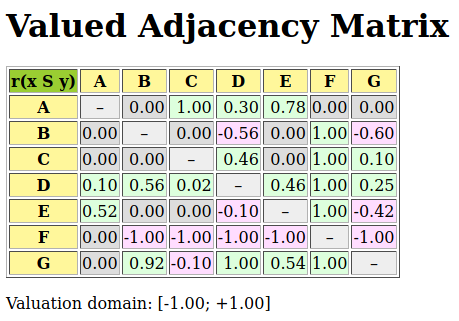
\includegraphics[width=7cm]{Figures/4-2-officeChoiceOutranking.png}
\caption[Bipolar-valued adjacency matrix]{\emph{Bipolar-valued adjacency matrix}. In the resulting outranking relation we may notice, on the one hand, that Alternative \texttt{D} is \emph{positively outranking} all other potential office locations. On the other hand, alternatives \texttt{A} (the most expensive) and \texttt{C} (the cheapest) are \emph{not outranked} by any other location}
\label{fig:4.2}       % Give a unique label
\end{figure}

Alternative \texttt{D} gives a \Condorcet winner\footnote{See Chapter~\ref{sec:7} on computing the winner of an election.}, whereas alternatives \texttt{A} (the most expensive) and \texttt{C} (the cheapest) give in fact \emph{weak} \Condorcet winners.\index{computeCondorcetWinners@\texttt{computeCondorcetWinners()}}\index{computeWeakCondorcetWinners@\texttt{computeWeakCondorcetWinners()}}
\begin{lstlisting}
>>> bod.computeCondorcetWinners()
 ['D']
>>> bod.computeWeakCondorcetWinners()
 ['A', 'C', 'D']
\end{lstlisting}

From theory, we know that outranking digraphs are \emph{weakly complete}\index{weakly complete}, i.e. for all $x$ and $y$ in $X$, $r(x \succsim y)\, <\, 0.0$ implies that $r(y \succsim x)\, \geqslant \, 0.0$. And, they verify the \emph{coduality principle}\index{coduality principle}:  $r(x \not\succsim y) \; = \; r(y \succnsim x)$ \citep{BIS-2013}.\footnote{Not to be confused with the dual graph of a plane graph \texttt{g} that has a vertex for each face of \texttt{g}. Here we mean the \emph{less than} (strict converse) relation corresponding to a \emph{greater or equal} relation, or the \emph{less than or equal} relation corresponding to a (strict) \emph{better than} relation.}

\begin{definition}[Strict outranking situation]\label{def:strictOutranking}\index{outranking!strict situation}

\noindent For two potential decision alternatives $x$ and $y$, ``$x$ \emph{strictly outranks} alternative $y$'', denoted $(x \succnsim y)$, when ``$x$ \emph{outranks} alternative $y$'' ($(x \succsim y) > 0.0$) and ``$y$ \emph{does not outrank} alternative $x$'' ($(y \succsim x) < 0.0$).
\end{definition}

Following from the coduality principle, the strict outranking digraph \texttt{bodcd} is build from the outranking digraph \texttt{bod} with a codual transform\index{codual transform} (see Sec.~\ref{sec:2.6}).
\begin{lstlisting} 
>>> bodcd = ~(-bod)  # codual tranform
>>> bodcd
*------- Object instance description ------*
Instance class       : BipolarOutrankingDigraph
Instance name        : converse-dual-rel_officeChoice
Actions              : 7
Criteria             : 7
Size                 : 10
Determinateness (%)  : 72.38
Valuation domain     : [-1.00;1.00]
\end{lstlisting}


\section{Designing a best choice recommender system}
\label{sec:4.4}

Solving a best-choice problem consists traditionally in finding \emph{the} unique best decision alternative. We adopt here instead a modern recommender system’s approach which shows a non empty subset of decision alternatives which contains by construction the potential best alternative(s).

The five \emph{pragmatic principles} for computing such a \emph{best-choice recommendation} (BCR) are the following:
\begin{itemize}[leftmargin=1cm,listparindent=0em]
\item [\texttt{P1}:] \emph{Elimination for well motivated reasons}; each eliminated alternative has to be strictly outranked by at least one alternative in the BCR.
\item [\texttt{P2}:] \emph{Minimal size}; the BCR must be as limited in cardinality as possible.
\item [\texttt{P3}:] \emph{Efficient and informative}; The BCR must not contain a self-contained sub-recommendation.
\item [\texttt{P4}:] \emph{Effectively better}; the BCR must not be ambiguous in the sense that it may not be both a first choice as well as a last choice recommendation.
\item [\texttt{P5}:] \emph{Maximally determined}; the BCR is, of all potential best-choice recommendations, the most determined one in the sense of the epistemic characteristics of the bipolar-valued outranking relation.
\end{itemize}

Let $X$ be the set of potential decision alternatives. Let $Y$ be a non empty subset of $X$, called a \emph{choice} in the strict outranking digraph $G(X,r(\succnsim )$. We can now qualify a BCR $Y$ in following terms:
\begin{itemize}[leftmargin=0.5cm,listparindent=0em]
\item [-] $Y$ is called strictly \emph{outranking} (resp. \emph{outranked}) when for all not selected alternative $x$ there exists an alternative $y \in X$ retained such that $r(y \succnsim x) > 0.0$ (resp. $r(y \precsim x) > 0.0$). Such a choice verifies principle \texttt{P1}.
\item [-] $Y$ is called \emph{weakly independent} when for all $x \neq y$ in $Y$ we observe $r(x \succnsim y) \leq 0.0$. Such a choice verifies principles \texttt{P3} (\emph{internal stability}).
\item [-] $Y$ is conjointly a strictly \emph{outranking} (resp. \emph{outranked}) \textbf{and} \emph{weakly independent} choice. Such a choice is called an \emph{initial} (resp. \emph{terminal}) \emph{prekernel}\footnote{See Chap.~\ref{sec:17} on computing kernels in digraphs}. The initial prekernel now verifies principles \texttt{P1}, \texttt{P2}, \texttt{P3} and \texttt{P4}. 
\item [-] To finally verify principle \texttt{P5}, we recommend among all potential initial prekernels, a \emph{most determined} one, i.e. a strictly \emph{outranking} and \emph{weakly independent} choice supported by the highest criteria significance. And in this most determined initial prekernel we eventually retain the alternative(s) that are included with highest criteria significance\footnote{See Sec.~\ref{sec:17.6}}.
\end{itemize}

Mind that a given strict outranking digraph may not always admit prekernels. This is the case when the digraph contains chordless circuits of odd length (see Chap.~\ref{sec:17}). Luckily, our strict outranking digraph \texttt{bodcd} here does not show any chordless outranking circuits; a fact we can check with the \texttt{computeChordless\-Cir\-cuits()} method\index{computeChordlessCircuits@\texttt{computeChordlessCircuits()}} followed by the \texttt{showChordlessCircuits()} method\index{showChordlessCircuits@\texttt{showChordlessCircuits()}}\footnote{The \texttt{computeChordlessCircuits()} and \texttt{showChordlessCircuits()} methods are separate because there are various methods available for enumerating the chordless circuits in a digraph \citep{BIS-2010}.}.
\begin{lstlisting}
>>> bodcd.computeChordlessCircuits()
  []  
>>> bodcd.showChordlessCircuits()
  No circuits observed in this digraph.
\end{lstlisting}

When observing chordless odd outranking circuits, we need to break them open with the \texttt{BrokenCocsDigraph} class at their weakest link, before enumerating the prekernels. \citep{BIS-2021b}.\index{BrokenCocsDigraph@\texttt{BrokenCocsDigraph} class}

We are ready now for building a best best choice recommendation.

\section{Computing the \Rubis best choice recommendation}
\label{sec:4.5}

The \texttt{showBestChoiceRecommendation()} method\index{showBestChoiceRecommendation@\texttt{showBestChoiceRecommendation()}} computes the \Rubis best choice recommendation directly from the outranking digraph $bod$. By default this method is operating on the \emph{codual} (strict) outranking digraph where chordless odd circuits have been bropen up (see the \texttt{CoDual} and \texttt{BrokenCocs} parameters in List.~\vref{list:4.4} Line~\ref{line:4.4.2}):
\begin{lstlisting}[caption={Computing the best choice recommendation},label=list:4.4]
>>> bod.showBestChoiceRecommendation(\
...              CoDual=True, BrokenCocs=True # default settings\ §\label{line:4.4.2}§
...              ChoiceVector = True)   §\label{line:4.4.3}§
  * --- First and last choice recommendation(s) ---*
    (in decreasing order of determinateness)   
    Credibility domain: [-1.00,1.00]
    === >> potential first choice(s)
    * choice              : ['A', 'C', 'D'] §\label{line:4.4.8}§
      independence        : 0.00
      dominance           : 0.10
      absorbency          : 0.00
      covering (%)        : 41.67
      determinateness (%) : 50.59
      - characteristic vector = {
        'D': +0.02, 'G': 0.00, 'C': 0.00, 'A': 0.00, §\label{line:4.4.15}§
        'F': -0.02, 'E': -0.02, 'B': -0.02, } §\label{line:4.4.16}§
    === >> potential last choice(s) 
    * choice              : ['A', 'F'] §\label{line:4.4.18}§
      independence        : 0.00
      dominance           : -0.52
      absorbency          : 1.00
      covered (%)         : 50.00
      determinateness (%) : 50.00
      - characteristic vector = {
        'G': 0.00, 'F': 0.00, 'E': 0.00, 'D': 0.00, §\label{line:4.4.25}§
        'C': 0.00, 'B': 0.00, 'A': 0.00, }          §\label{line:4.4.26}§
\end{lstlisting}				  

It is interesting to notice in Line~\ref{line:4.4.8} above that the \Rubis \emph{first choice recommendation} consists actually in the previously mentioned set of weak \Condorcet winners\index{Condorcet@\Condorcet!winner}: \texttt{A}, \texttt{C} and \texttt{D} (see Fig.~\vref{fig:4.2}). In the corresponding prekernel characteristic vector (see Lines~\ref{line:4.4.3},~\ref{line:4.4.15} and Sec.~\ref{sec:17.6}), representing the bipolar credibility degree with which each alternative may indeed be included in, or excluded from this recommendation, we find that alternative \texttt{D} is the only positively validated one, whereas both extreme alternatives --\texttt{A} (the most expensive) and \texttt{C} (the cheapest)-- stay in an indeterminate situation (see \citealp{BIS-2006a,BIS-2006b}). They may \emph{be or not be} potential best choices. Notice furthermore that compromise alternative \texttt{G}, while not actually being included in this strictly outranking prekernel, shows as well an indeterminate situation with respect to \emph{being or not being} recommended as potential best choice. Alternatives \texttt{B}, \texttt{E} and \texttt{F} are all negatively included, i.e. positively excluded, from this best choice recommendation (see Line~\ref{line:4.4.16}).

To inspect why alternative \texttt{D} is the only positive best choice recommendation, we shall compare now the evaluations of alternatives \texttt{D} and \texttt{G} in a pairwise perspective\index{showPairwiseComparison@\texttt{showPairwiseComparison()}}.
\begin{lstlisting}[caption={Inspecting pairwise comparison between alternatives \texttt{G} and \texttt{D}},label=list:4.5,basicstyle=\ttfamily\scriptsize]
>>> bod.showPairwiseComparison('G','D')
 *------------  pairwise comparison ----*
  Comparing actions : ('G', 'D')
  crit.  wght.    g(x)      g(y)    diff.  |   ind.    pref.  concord. 
  ====================================================================
   Costs 45.00 -12000.00 -14100.00 +2100.00 | 1000.00 2500.00  +45.00  
   Comf.  6.00     50.00     30.00   +20.00 |   10.00   20.00   +6.00 
   Park.  3.00     80.00     90.00   -10.00 |   10.00   20.00   +3.00 
   Prox. 32.00     60.00     70.00   -10.00 |   10.00   20.00  +32.00 
   Stdg. 23.00     20.00     30.00   -10.00 |   10.00   20.00  +23.00 
   Visi. 26.00    100.00     50.00   +50.00 |   10.00   20.00  +26.00 
   Spac. 10.00     50.00     55.00    -5.00 |   10.00   20.00  +10.00
   =====================================================================
    Valuation in range: -145.00 to +145.00; global concordance: +145.00
\end{lstlisting}

In Listing~\vref{list:4.5}, we notice that, with the given preference discrimination thresholds, alternative \texttt{G} is actually \emph{certainly at least as well evaluated as} alternative \texttt{D}:  $r(G \succsim D)\, = \, +145/145\, =\, +1.0$.

Yet, we must as well acknowledge in Listing~\vref{list:4.6}, that the cheapest alternative \texttt{C} is in fact \emph{strictly outranking} alternative \texttt{G}:  $r(C \succsim G)\, =\, +15/145\, >\, 0.0$, and $r(G \succsim C)\, =\, -15/145 \,<\, 0.0$.
\begin{lstlisting}[caption={Inspecting pairwise comparison between alternatives \texttt{C} and \texttt{G}},label=list:4.6,basicstyle=\ttfamily\scriptsize]
>>> bod.showPairwiseComparison('C','G')
 *------------  pairwise comparison ----*
  Comparing actions : (C,G)/(G,C)
  crit. wght.   g(x)     g(y)      diff.  |   ind.   pref.       (C,G)/(G,C)
   ==========================================================================
   'C'   45.00 -6700.00 -12000.00 +5300.00 | 1000.00 2500.00    +45.00/-45.00 
   'Cf'   6.00    10.00     50.00   -40.00 |   10.00   20.00     -6.00/ +6.00 
   'P'    3.00   100.00     80.00   +20.00 |   10.00   20.00     +3.00/ -3.00 
   'Pr'  32.00    80.00     60.00   +20.00 |   10.00   20.00    +32.00/-32.00 
   'St'  23.00     0.00     20.00   -20.00 |   10.00   20.00    -23.00/+23.00 
   'V'   26.00    70.00    100.00   -30.00 |   10.00   20.00    -26.00/+26.00 
   'W'   10.00     0.00     50.00   -50.00 |   10.00   20.00    -10.00/+10.00
                                                               --------------
    Valuation in range: -145 to +145;      r(C >= G)/r(G >= c): +15.00/-15.00
\end{lstlisting}
\begin{figure}[ht]
\sidecaption[t]
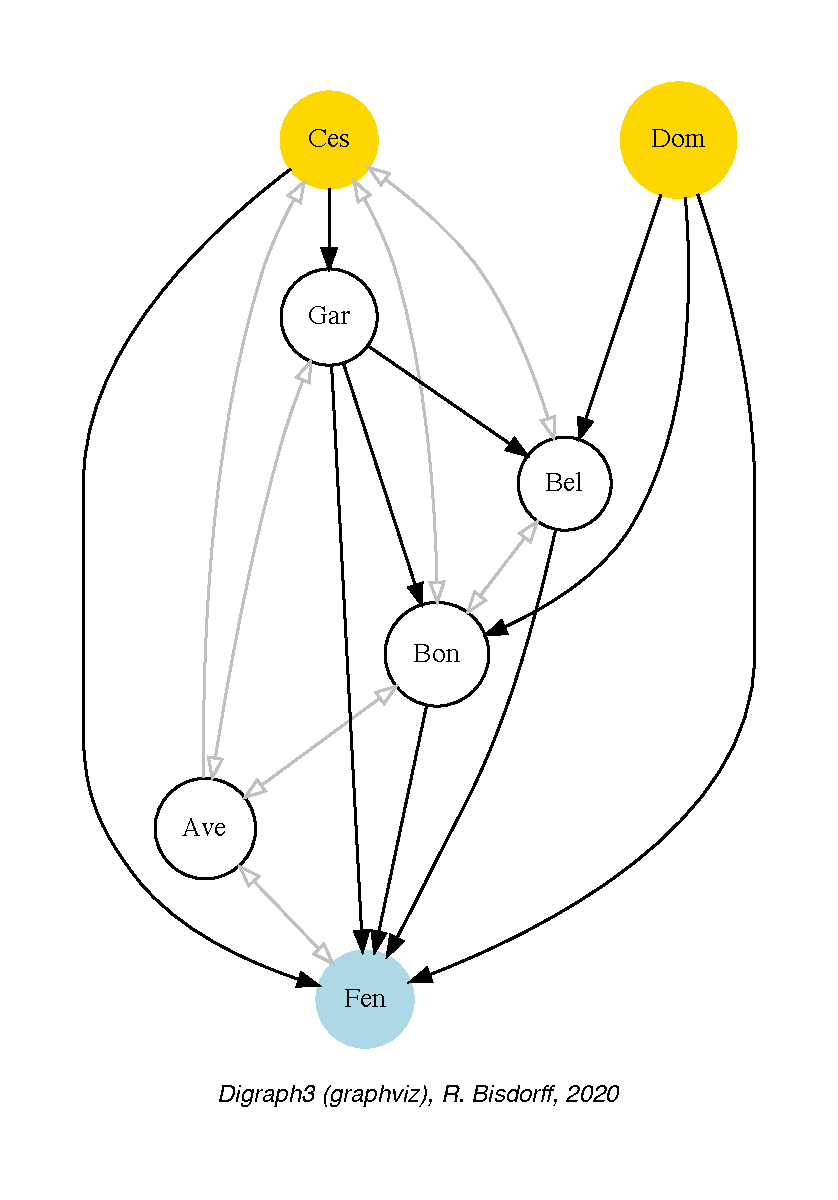
\includegraphics[width=6cm]{Figures/4-3-bestOfficeChoice.pdf}
\caption[Best office choice recommendation from strict outranking digraph]{\emph{Best office choice recommendation from strict outranking digraph}. Notice that location \texttt{A} (\emph{Ave}) (the most expensive) is appearing \emph{incomparable} to all the other alternatives}
\label{fig:4.3}       % Give a unique label
\end{figure}

Let us finally notice in Listing~\vref{list:4.4} Line~\ref{line:4.4.18} that both alternatives \texttt{A} and \texttt{F} are reported as potential last choice recommendation. Yet, this last choice recommendation appears to be globally indeterminate (Lines~\ref{line:4.4.25}-\ref{line:4.4.26}). This confirms the \emph{incomparability} status of alternative \texttt{A} (see Fig.~\vref{fig:4.3}).
\begin{lstlisting}
>>> bodcd.exportGraphViz(fileName='bestOfficeChoice',\
...                    firstChoice=['C','D'],\
...                    lastChoice=['F'])
  *---- exporting a dot file for GraphViz tools ---------*
   Exporting to bestOfficeChoice.dot
   dot -Grankdir=BT -Tpng bestOfficeChoice.dot \
                    -o bestOfficeChoice.png
\end{lstlisting}

\section{Weakly ordering the outranking digraph}
\label{sec:4.6}

To get a global insight in the overall strict outranking situations, we may use the \texttt{RankingByChoosingDigraph}\index{RankingByChoosingDigraph@\texttt{RankingByChoosingDigraph} class} class imported from the \texttt{transitive\-Digraphs}\index{transitiveDigraphs@\texttt{transitiveDigraphs} module} module for computing a \emph{ranking-by-choosing} result from the codual, i.e. the strict outranking digraph instance \texttt{bodcd} (see above). If the computing node supports multiple processor cores, \emph{first} and \emph{last} choosing iterations may be run in parallel (see Line~\ref{line:4.7.4} in List.~\vref{list:4.7}).
\begin{lstlisting}[caption={Ranking-by-choosing the outranking digraph},label=list:4.7]
>>> from transitiveDigraphs import\
...                  RankingByChoosingDigraph
>>> rbc = RankingByChoosingDigraph(bodcd)
 Threading ... # multiprocessing if 2 cores are available §\label{line:4.7.4}§
 Exiting computing threads
>>> rbc.showRankingByChoosing()
 Ranking by Choosing and Rejecting
    1st ranked ['D']
       2nd ranked ['C', 'G']
       2nd last ranked ['B', 'C', 'E']
    1st last ranked ['A', 'F']
>>> rbc.exportGraphViz('officeChoiceRanking')
 *---- exporting a dot file for GraphViz tools ---------*
  Exporting to officeChoiceRanking.dot
  dot -Grankdir=TB -Tpng officeChoiceRanking.dot\
                   -o officeChoiceRanking.png
\end{lstlisting}
\begin{figure}[ht]
\sidecaption[t]
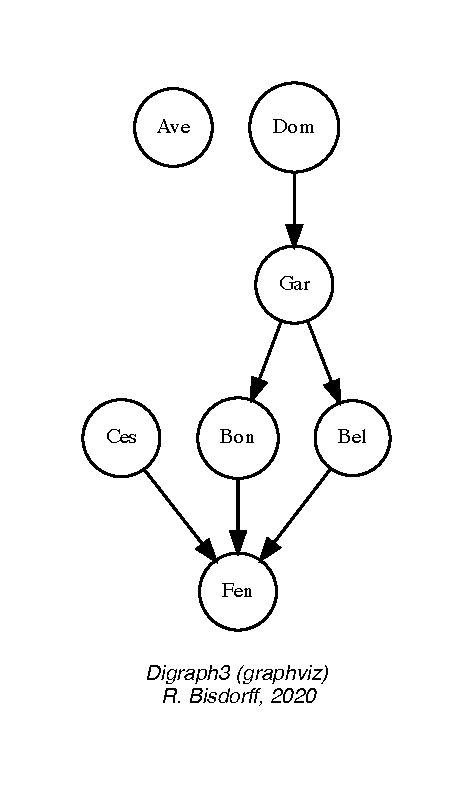
\includegraphics[width=5cm]{Figures/4-4-officeChoiceRanking.pdf}
\caption[Ranking-by-choosing the potential office locations]{\emph{Ranking-by-choosing the potentail office locations}. In this \emph{ranking-by-choosing} method, where we operate the \emph{epistemic fusion} of iterated (strict) first and last choices, compromise alternative \texttt{Dom} is now ranked before compromise alternative \texttt{Gar}. The overall partial ordering result shows again the important fact that the most expensive location \texttt{Ave}, and the cheapest location \texttt{Ces}, due to their contradictory performances, appear both \emph{incomparable} with most of the other alternatives.} 
\label{fig:4.4}       % Give a unique label
\end{figure}

The best choice recommendation hence depends on the very importance the CEO is attaching to each of his decision objectives. In the given setting here, where he considers that \emph{maximising the future turnover} is the most important objective followed by \emph{minimising the Costs} and, less important, \emph{maximising the working conditions}, location \texttt{D} represents actually the \emph{best compromise}. However, if \emph{Costs} do not play much a role, it would be perhaps better to decide to move to the most advantageous location \texttt{A}; or if, on the contrary, \emph{Costs} do matter a lot, moving to the cheapest alternative \texttt{C} could definitely represent a more convincing recommendation. 

It might be worth editing the criteria significance weights in the\\
\texttt{officeChoice.py} data file in such a way that:
\begin{itemize}[topsep=2pt]
\item All three decision objectives are considered \emph{equally important}, and
\item All criteria under each objective are considered \emph{equi-significant}.
\end{itemize}

What will become the best choice recommendation under this working hypothesis?\footnote{See also the notes of Lecture 7 from the MICS Algorithmic Decision Theory course \citep{ADT-L7}.} 

%\vspace{1cm}
\vspace{\baselineskip}
In the next Chapter~\ref{sec:5} we precisely show how to edit a new performance tableau from a given template file. 

%%%%%%%%%%%%%%%%%%%%%%%%%%%%%%%%%%%%
\phantomsection
\addcontentsline{toc}{section}{Notes}
\section*{Notes}

Following a seminar presentation in 2005 at the LAMSADE\footnote{Laboratoires d'Analyse et de Modélisation de Systèmes d'Aide à la Décision, Université Paris-Dauphine, UMR 7243 CNRS}, where the author promoted the use of kernels of the outranking digraph as suitable candidates for delivering best choice recommendations \citep{BIS-2005}, a critical discussion started about the methodological requirement for a convincing best choice recommendation to be internally stable (pragmatic principle \texttt{P3}). \emph{Denis Bouyssou}\index{Bouyssou@\emph{D. Bouyssou}} illustrated his doubts with the potential outranking digraph shown in Figure~\vref{fig:4.5}.
\begin{figure}[ht]
\sidecaption[t]
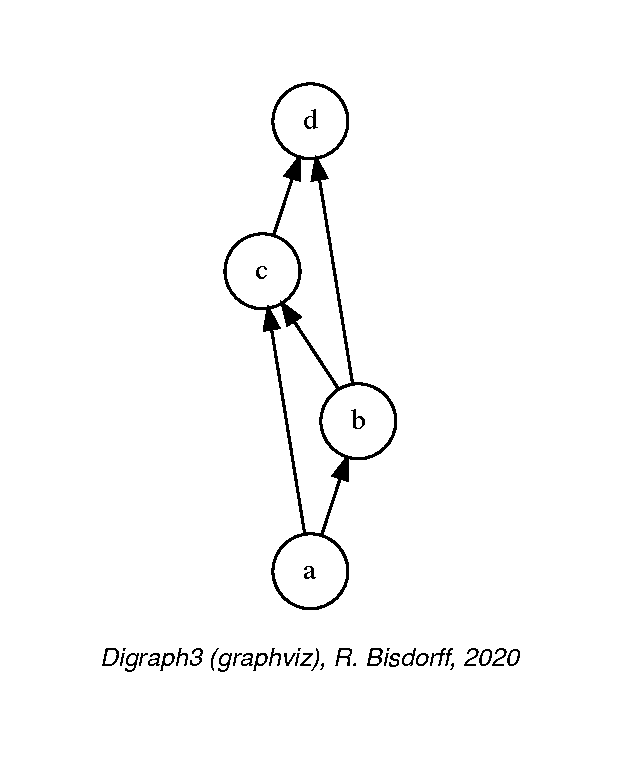
\includegraphics[width=6cm]{Figures/4-5-bouyssou11Oct05crisp.pdf}
\caption[The internal stability of a best choice recommendation in question]{\emph{The internal stability of a best choice recommendation in question}. The only kernel of this digraph is the pair $\{\mathtt{a},\mathtt{d}\}$; yet, it is an ambiguous recommendation, as $\{\mathtt{a},\mathtt{d}\}$ is conjointly an outranking and outranked choice. If the instability of the best choice recommendation is, however, not considered a problem then the choice $\{\mathtt{a},\mathtt{b}\}$ shows the most convincing strict outranking quality and could be considered in priority for recommendation as potential best choice candidates}
\label{fig:4.5}       % Give a unique label
\end{figure}

His commentary was the following: Adding alternative \texttt{d} to the set of potential best choice candidates is not convincing as there exists in the given digraph the node \texttt{b}, which is better evaluated than \texttt{d}. The argument that the incomparability between \texttt{a} and \texttt{d} should favour \texttt{d} as potential best choice is interesting but another hypothesis could be that \texttt{b} perhaps outranks \texttt{a}. In this latter case, it seams clear that the actual best choice recommendation should be reduced to node \texttt{b}, unless one disposes of other information, like a performance tableau and/or the actual computation method of the outranking situations. In any case, one has to be very clear about the available information when judging a best choice procedure.

It became thereafter obvious for us all that both the lack of a specific performance tableau as well as the lack of a precisely defined algorithm for computing valid outranking situations do not allow to judge if a given digraph does indeed model a potential outranking relation. In our present bipolar-valued epistemic approach, a valid outranking digraph instance, following from a given performance tableau and the disjunctive epistemic fusion construction of the outranking relation (see Chap.~\ref{sec:3}), will necessarily verify the weak completeness condition and the coduality principle. As a consequence, incomparability situations are now modelled by epistemic indeterminateness not by the actual absence of a reciprocal outranking relation.

The digraph put forward by \emph{D. Bouyssou} in the October 2005 discussion is not weakly complete --node \texttt{a} is not outranking node \texttt{d} and vice versa-- and does hence not represent, in our present sense, a valid outranking digraph instance. Yet, it may be a partial tournament and as such it could be a strict outranking digraph, i.e. the asymmetric part --the codual-- of a valid outranking digraph. In this case, nodes \texttt{a} and \texttt{d} --the kernel of the strict outranking digraph-- would actually for sure outrank each other and, hence, represent both indifferently the natural best choice recommendation. However, in this not strict codual digraph, node \texttt{a} becomes also the unique \Condorcet winner --outranking for sure all other nodes-- and gives hence the evident unique best choice recommendation.

Only after 2013, when the weak completeness and the coduality properties of the outranking digraph were discovered, became it obvious that the initial prekernels of the strict outranking digraph, coupled with the solution of the corresponding kernel equation system, were in fact delivering the most convincing best choice recommendations (see Chap.~\ref{sec:17}, Sec.~\ref{sec:20.4} and \citealp{BIS-2013}). It stays an interesting open mathematical problem to show (or not) that both necessary conditions: --weak completeness and coduality-- are also sufficient for qualifying any bipolar-valued digraph as potential instance of an outranking digraph.


%%%%%%% The chapter bibliography
%\normallatexbib
%\clearpage
%\phantomsection
%\addcontentsline{toc}{section}{Chapter Bibliography}
%\chapter{Building a best choice recommendation}
\label{sec:4}

\abstract*{  This chapter presents the \Rubis best choice recommender system. Our approach is illustrated with building a best office site recommendation. We show how to explore the given performance tableau and compute the corresponding outranking digraph. After presenting the pragmatic principles that govern our best choice recommendation algorithm we solve the best office-location choice problem.}

\begin{quotation}
  ``... \emph{The goal of our research was to design a resolution method} ... \emph{that is easy to put into practice, that requires as few and reliable hypotheses as possible, and that meets the needs} [of the decision maker]...''

  --\citep*{ROY-1966}\index{Roy@\textsl{B. Roy}}.
\end{quotation}
\vspace{1cm}

\abstract{ This chapter presents the \Rubis best choice recommender system. Our approach is illustrated with a best office location selection problem. We show how to explore the given performance tableau and compute the corresponding outranking digraph. After presenting the pragmatic principles that govern our best choice recommendation algorithm we solve the best office location choice problem.}

\section{What office-location to choose?}
\label{sec:4.1}

A SME, specialised in printing and copy services, has to move into new offices, and its CEO has gathered seven \emph{potential new office locations} (see Table~\vref{tab:4.1}).
\begin{table}[ht]
\caption{The potential new office locations}
\label{tab:4.1}       % Give a unique label
\begin{center}
  %\begin{small}
    \begin{tabular}{c|l|l|l}
      \svhline\noalign{\smallskip}
      ID & Name & Address & Comment\\
      \noalign{\smallskip}\hline\noalign{\smallskip}
    A &   Ave  &  Avenue de la liberté &  High standing city center\\
    B &   Bon  &  Bonnevoie &             Industrial environment\\
    C &   Ces  &  Cessange &              Residential suburb location\\
    D &   Dom  &  Dommeldange &           Industrial suburb environment\\
    E &   Bel  &  Esch-Belval &           New and ambitious urbanisation far from the city\\
    F &   Fen  &  Fentange &              Out in the countryside\\
      G &   Gar  &  Avenue de la Gare &     Main city shopping street\\
      \noalign{\smallskip}\hline
    \end{tabular}
  %\end{small}
\end{center}
\end{table}

Three \emph{decision objectives}, in order of decreasing importance, are guiding the CEO's choice:
\begin{enumerate}[leftmargin=1cm]
\item \emph{maximise} the future turnover of the SME,
\item \emph{minimise} the future yearly costs induced by the moving,
\item \emph{maximise} the new working conditions.
\end{enumerate}

The decision consequences to take into account for evaluating the potential new office locations with respect to each one of the three objectives are modelled by the \emph{family of performance criteria} \footnote{See \citealp{ROY-2000}} shown in Table~\vref{tab:4.2} below.
\begin{table}[ht]
\caption{The family of performance criteria}
\label{tab:4.2}       % Give a unique label
\begin{center}
    \begin{tabular}{l|c|c|c|l}
      \svhline\noalign{\smallskip}
      Objective & ID & Name & Weight & Comment\\
      \noalign{\smallskip}\hline\noalign{\smallskip}
    Yearly costs  &       Ct &   Costs &  45 &     Annual rent, charges, and cleaning\\
    \             &  \      & \        &  \ & \ \\
    Future turnover   &   Pr  & Proximity  & 32 & Distance from town center\\
    Future turnover   &   V  &  Visibility & 26 & Circulation of potential customers \\
    Future turnover   &   St &   Standing & 23 &   Image and presentation\\
    \                 &   \   & \          &  \ & \  \\
    Working conditions &  W  &  Space   &   10 &  Working space\\
    Working conditions &  Cf &  Comfort  &  6 &  Quality of office equipment\\
    Working conditions &  P  &  Parking  &  3 &  Available parking facilities\\
      \noalign{\smallskip}\hline
    \end{tabular}   
  \end{center}
\end{table}

In Table~\vref{tab:4.2} we notice that the \emph{Costs} criterion admits the highest significance weight ($45$), followed by the \emph{Future turnover} criteria $(32, 26, 23)$, The \emph{Working conditions} criteria are the less significant $(10, 6, 3)$ \footnote{These criteria weights were supposedly established with a swing weighing MCDA method \citep{KEE-1976}.}. It follows that the CEO considers \emph{maximising the future turnover} the most important objective ($(32 + 26+ 23) = 81$), followed by minimising the future yearly costs ($45$), and less important, \emph{maximising working conditions} ($(10 + 6 + 3) = 19$). 

The evaluations of the seven potential new locations on each performance criterion are gathered in a \emph{performance table} shown in Table~\vref{tab:4.3}.
\begin{table}[ht]
\caption{Performance evaluations of the potential office locations}
\label{tab:4.3}       % Give a unique label
\begin{center}
    \begin{tabular}{l|c|c|c|c|c|c|c}
      \svhline\noalign{\smallskip}
    Criterion  &    A  &      B &       C &       D &       E &        F &        G\\
       \noalign{\smallskip}\hline\noalign{\smallskip}

    Costs      &   35.0K€ &  17.8K€  & 6.7K€  &  14.1K€ &  34.8K€ &  18.6K€ &  12.0K€\\
    \          &   \      &  \     &   \     &   \    &    \    &    \    &    \ \\
    Proximity     &   100    &  20 &      80    &   70    &   40    &   0    &    60 \\
    Visibility     &   60     &  80  &     70    &   50    &   60    &   0    &    100 \\
    Standing      &   100   &   10   &    0     &   30    &   90    &   70   &    20 \\
    \           &   \     &   \    &    \     &   \     &   \     &   \    &    \  \\
    Working space      &   75    &   30   &    0     &   55    &   100   &   0    &    50  \\
    Working comfort      &   0     &   100  &    10    &   30    &   60    &   80   &    50 \\
    Parking     &   90    &   30   &    100   &   90    &   70    &   0    &    80 \\
      \noalign{\smallskip}\hline
    \end{tabular}
  \end{center}
\end{table}
All criteria, except the \emph{Costs} Criterion, admit for evaluation a qualitative satisfaction scale from $0\%$ (weakest) to $100\%$ (highest). One may thus notice that location \texttt{A} (\emph{Ave}) is the most expensive, but also $100\%$ satisfying the \emph{Proximity} as well as the  \emph{Standing} criterion. Whereas location \texttt{C} (\emph{Ces}) is the cheapest one; providing however no satisfaction at all on both the \emph{Standing} and the \emph{Working Space} criteria.

Concerning yearly costs, we suppose that the CEO is indifferent up to a performance difference of $1000.00$€, and he actually prefers a location when there is at least a positive difference of $2500.00$€. The evaluations observed on the six qualitative criteria (measured in percentages of satisfaction) are very subjective and rather imprecise. The CEO is hence \emph{indifferent} up to a satisfaction difference of $10\%$, and he claims a significant \emph{preference} when the satisfaction difference is at least of $20\%$.  Furthermore, a satisfaction difference of $80\%$ represents for him a \emph{considerably large} performance difference, triggering the case given a \emph{polarisation} of the preferential situation \citep{BIS-2013}. 

In view of Table~\vref{tab:4.3}, what is now the office location we may recommend to the CEO as \textbf{best choice}?

\section{The given performance tableau}
\label{sec:4.2}


The file \texttt{officeChoice.py}, stored in the \texttt{examples} directory of the \Digraph resources, provides a corresponding \texttt{PerformanceTableau}\index{PerformanceTableau@\texttt{PerformanceTableau} class} object. We can inspect its actual content with the computing resources provided by the \texttt{perfTabs} module \index{perfTabs@\texttt{perfTabs} module}.
\begin{lstlisting}[caption={Inspecting the \texttt{officeChoice} performance tableau.},label=list:4.1]
>>> from perfTabs import PerformanceTableau
>>> pt = PerformanceTableau('officeChoice')
>>> pt
 *------- PerformanceTableau instance description ------*
   Instance class     : PerformanceTableau
   Instance name      : officeChoice
   Actions            : 7
   Objectives         : 3
   Criteria           : 7
   NaN proportion (%) : 0.0
   Attributes         : ['name', 'actions', 'objectives',
                         'criteria', 'weightPreorder',
			 'NA', 'evaluation']
>>> pt.showPerformanceTableau()
 *----  performance tableau -----*
  Criteria|  'Ct'       'Cf'   'P'   'Pr'   'St'    'V'    'W'   
  Weights |  45.00      6.00   3.00  32.00  23.00  26.00  10.00    
  --------|----------------------------------------------------
   'Ave'  | -35000.00   0.00  90.00 100.00 100.00  60.00  75.00  
   'Bon'  | -17800.00 100.00  30.00  20.00  10.00  80.00  30.00  
   'Ces'  |  -6700.00  10.00 100.00  80.00   0.00  70.00   0.00  
   'Dom'  | -14100.00  30.00  90.00  70.00  30.00  50.00  55.00  
   'Bel'  | -34800.00  60.00  70.00  40.00  90.00  60.00 100.00  
   'Fen'  | -18600.00  80.00   0.00   0.00  70.00   0.00   0.00  
   'Gar'  | -12000.00  50.00  80.00  60.00  20.00 100.00  50.00  
\end{lstlisting}

We thus recover all the input data shown in Section~\ref{sec:4.1}. Notice that the \emph{negative} evaluations of the \emph{Costs} criterion indicate a negative preference direction: the \emph{lower} the costs, the \emph{better} it is.

The \texttt{showCriteria()}\index{showCriteria@\texttt{showCriteria()}} method evaluates the actual preference discrimination we observe on each performance criterion.
\begin{lstlisting}[caption={Inspecting the performance criteria.},label=list:4.2]
>>> pt.showCriteria(IntegerWeights=True)
 *----  criteria -----*
  Ct 'Costs'
   Preference direction: min
   Scale = (0.00, 50000.00)
   Weight = 45
   Threshold ind : 1000.00 + 0.00x ;  percentile:  9.52 §\label{line:4.2.7}§
   Threshold pref : 2500.00 + 0.00x ; percentile: 14.29 §\label{line:4.2.8}§
  Cf 'Comfort'
   Preference direction: max
   Scale = (0.00, 100.00)
   Weight = 6
   Threshold ind : 10.00 + 0.00x ;  percentile:   9.52 §\label{line:4.2.13}§
   Threshold pref : 20.00 + 0.00x ; percentile:  28.57 §\label{line:4.2.14}§
   Threshold veto : 80.00 + 0.00x ; percentile:  90.48 §\label{line:4.2.15}§
   ...
   ...
\end{lstlisting}

On the \emph{Costs} criterion, $9.5\%$ of the performance differences are considered insignificant and $14.3\%$ below the preference discrimination threshold (see Lines~\ref{line:4.2.7}--\ref{line:4.2.8} in List.~\vref{list:4.2}). On the qualitative \emph{Comfort} criterion, we observe again $9.5\%$ of insignificant performance differences (line~\ref{line:4.2.13}). Due to the imprecision in the subjective evaluations, we notice here $28.6\%$ of performance differences below the preference discrimination threshold (Line~\ref{line:4.2.14}). Furthermore, $100.0 - 90.5 = 9.5\%$ of the performance differences are judged \emph{considerably large} (Line~\ref{line:4.2.15}) and will trigger hence a polarisation of the concerned outranking situations \citep{BIS-2013}. Same information is available for all the other criteria. 
 
A colourful comparison of all the evaluations is shown in Fig.~\vref{fig:4.1} by the \emph{heatmap}\index{showHTMLPerformanceHeatmap@\texttt{showHTMLPerformanceHeatmap()}} statistics, illustrating the respective quantile class of each evaluation. As the set of potential alternatives is tiny, we choose here a classification into performance quintiles.
\begin{lstlisting}
>>> pt.showHTMLPerformanceHeatmap(colorLevels=5,\
...                              rankingRule=None)
\end{lstlisting}
    \begin{figure}[ht]
%\sidecaption
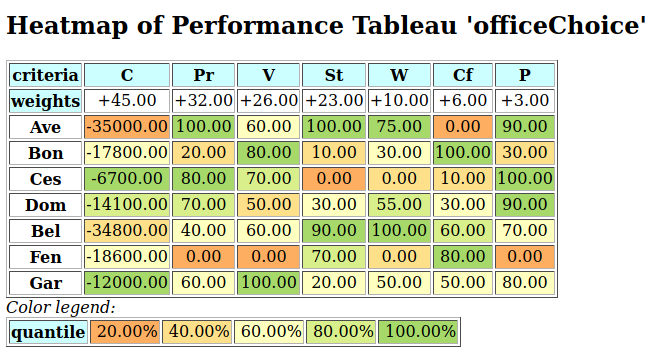
\includegraphics[width=0.8\hsize]{Figures/4-1-officeChoiceHeatmap.png}
\caption{Unranked heatmap of the office choice performance tableau}
\label{fig:4.1}       % Give a unique label
\end{figure}

Location \texttt{Ave} shows extreme and contradictory evaluations: highest \emph{Costs} and no \emph{Working Comfort} on the one hand, and total satisfaction with respect to \emph{Standing}, \emph{Proximity} and \emph{Parking facilities} on the other hand. Similar, but opposite, situation is given for location \texttt{Ces}: unsatisfactory \emph{Working Space}, no \emph{Standing} and no \emph{Working Comfort} on the one hand, and lowest \emph{Costs}, best \emph{Proximity} and \emph{Parking facilities} on the other hand. Contrary to these contradictory alternatives, we observe two appealing compromise alternatives: locations \texttt{Dom} and \texttt{Gar}. Finally, location \texttt{Fen} is clearly the less satisfactory alternative of all.

To help now the CEO choosing the best office location, we are going to compute pairwise outranking situations on the set of potential decision alternatives (see \citealp{BIS-2013}).

\section{Computing the outranking digraph}
\label{sec:4.3}

\begin{definition}[Outranking situation]\label{def:outranking}\index{outranking!situation}

\noindent For two potential decision alternatives $x$ and $y$:
\begin{itemize}[leftmargin=0.5cm,rightmargin=0.5cm]
\item ``Alternative $x$ \emph{outranks} alternative $y$'', denoted $(x \succsim y)$, is given when:
   \begin{enumerate}[nosep]
     \item A \emph{majority} of criteria significance warrants that alternative $x$ is \emph{at least as well evaluated as} alternative $y$, and
     \item \emph{No considerable} negative performance difference is observed on any criterion.      
    \end{enumerate}
\item ``Alternative $x$ \emph{does not outrank} $y$'', denoted $(x \not\succsim y)$, is given when:
   \begin{enumerate}[nosep]
    \item Only a \emph{minority} of criteria significance warrants that alternative $x$ is \emph{at least as well evaluated as} alternative $y$, and
    \item \emph{No considerable} positive performance difference is observed on any criterion. 
    \end{enumerate}
\item Otherwise, the outranking situation between alternatives $x$ and $y$ is considered to be \emph{indeterminate}.
\end{itemize}
\end{definition}

The credibility of each pairwise outranking situation, denoted $r(x \succsim y)$, is measured in a bipolar significance valuation $[-1.0, 1.0]$, where \emph{positive} terms $r(x \succsim y)\, >\, 0.0$ indicate a \emph{validated outranking}, and \emph{negative} terms $r(x \succsim y)\, <\, 0.0$ indicate an \emph{invalidated outranking}, i.e. a \emph{validated outranked} situation. The \emph{median} value $r(x \succsim y)\, = \,0.0$ represents an \emph{indeterminate} situation (see \citealp{BIS-2004a} and \citealp{BIS-2013}).   

For computing such a bipolar-valued binary outranking relation from the given performance tableau \texttt{pt}, we use the \texttt{BipolarOutrankingDigraph}\index{BipolarOutrankingDigraph@\texttt{BipolarOutrankingDigraph} class} class from the \texttt{outrankingDigraphs}\index{outrankingDigraphs@\texttt{outrankingDigraphs} module} module. The corresponding
\texttt{showHTMLRe\-lation\-Table()}\index{showHTMLRelationTable@\texttt{showHTMLRelationTable()}} method shows here the resulting bipolar-valued adjacency matrix in a system browser window (see Fig.~\vref{fig:4.2}).
\begin{lstlisting}[caption={Computing a bipolar-valued outranking digraph},label=list:4.3]
>>> from outrankingDigraphs import BipolarOutrankingDigraph
>>> bod = BipolarOutrankingDigraph(pt)
>>> bod.showHTMLRelationTable()
\end{lstlisting}
\begin{figure}[ht]
\sidecaption[t]
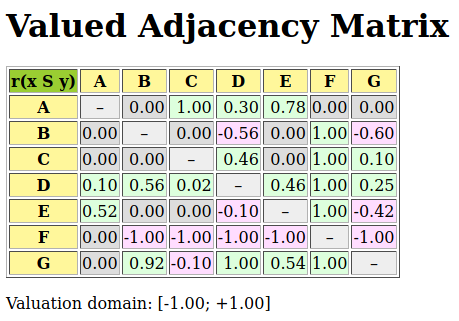
\includegraphics[width=7cm]{Figures/4-2-officeChoiceOutranking.png}
\caption[Bipolar-valued adjacency matrix]{\emph{Bipolar-valued adjacency matrix}\\ In the resulting outranking relation we may notice, on the one hand, that Alternative \texttt{D} is \emph{positively outranking} all other potential office locations. On the other hand, alternatives \texttt{A} (the most expensive) and \texttt{C} (the cheapest) are \emph{not outranked} by any other location.}
\label{fig:4.2}       % Give a unique label
\end{figure}

Alternative \texttt{D} gives a \Condorcet winner\footnote{See Chap.~\ref{sec:7} on computing the winner of an election.}, whereas alternatives \texttt{A} (the most expensive) and \texttt{C} (the cheapest) give in fact \emph{weak} \Condorcet winners.\index{computeCondorcetWinners@\texttt{computeCondorcetWinners()}}\index{computeWeakCondorcetWinners@\texttt{computeWeakCondorcetWinners()}}
\begin{lstlisting}
>>> bod.computeCondorcetWinners()
 ['D']
>>> bod.computeWeakCondorcetWinners()
 ['A', 'C', 'D']
\end{lstlisting}

From theory, we know that outranking digraphs are \emph{weakly complete}\index{weakly complete}, i.e. for all $x$ and $y$ in $X$, $r(x \succsim y)\, <\, 0.0$ implies that $r(y \succsim x)\, \geqslant \, 0.0$. And, they verify the \emph{coduality principle}\index{coduality principle}:  $r(x \not\succsim y) \; = \; r(y \succnsim x)$ \citep{BIS-2013}.\footnote{Not to be confused with the dual graph of a plane graph \texttt{g} that has a vertex for each face of \texttt{g}. Here we mean the \emph{less than} (strict converse) relation corresponding to a \emph{greater or equal} relation, or the \emph{less than or equal} relation corresponding to a (strict) \emph{better than} relation.}

\begin{definition}[Strict outranking situation]\label{def:strictOutranking}\index{outranking!strict situation}

\noindent For two potential decision alternatives $x$ and $y$, ``$x$ \emph{strictly outranks} alternative $y$'', denoted $(x \succnsim y)$, when ``$x$ \emph{outranks} alternative $y$'' ($(x \succsim y) > 0.0$) and ``$y$ \emph{does not outrank} alternative $x$'' ($(y \succsim x) < 0.0$).
\end{definition}

Following from the coduality principle, the strict outranking digraph \texttt{bodcd} is build from the outranking digraph \texttt{bod} with a codual transform\index{codual transform} (see Sect.~\ref{sec:2.6}).
\begin{lstlisting} 
>>> bodcd = ~(-bod)  # codual tranform
>>> bodcd
*------- Object instance description ------*
Instance class       : BipolarOutrankingDigraph
Instance name        : converse-dual-rel_officeChoice
Actions              : 7
Criteria             : 7
Size                 : 10
Determinateness (%)  : 72.38
Valuation domain     : [-1.00;1.00]
\end{lstlisting}


\section{Designing a best choice recommender system}
\label{sec:4.4}

Solving a best-choice problem consists traditionally in finding \emph{the} unique best decision alternative. We adopt here instead a modern recommender system’s approach which shows a non empty subset of decision alternatives which contains by construction the potential best alternative(s).

The five \emph{pragmatic principles} for computing such a \emph{best-choice recommendation} (BCR) are the following:
\begin{itemize}[leftmargin=1cm,listparindent=0em]
\item [\texttt{P1}:] \emph{Elimination for well motivated reasons}; each eliminated alternative has to be strictly outranked by at least one alternative in the BCR.
\item [\texttt{P2}:] \emph{Minimal size}; the BCR must be as limited in cardinality as possible.
\item [\texttt{P3}:] \emph{Efficient and informative}; The BCR must not contain a self-contained sub-recommendation.
\item [\texttt{P4}:] \emph{Effectively better}; the BCR must not be ambiguous in the sense that it may not be both a first choice as well as a last choice recommendation.
\item [\texttt{P5}:] \emph{Maximally determined}; the BCR is, of all potential best-choice recommendations, the most determined one in the sense of the epistemic characteristics of the bipolar-valued outranking relation.
\end{itemize}

Let $X$ be the set of potential decision alternatives. Let $Y$ be a non empty subset of $X$, called a \emph{choice} in the strict outranking digraph $G(X,r(\succnsim )$. We can now qualify a BCR $Y$ in following terms:
\begin{itemize}[leftmargin=0.5cm,listparindent=0em]
\item [-] $Y$ is called strictly \emph{outranking} (resp. \emph{outranked}) when for all not selected alternative $x$ there exists an alternative $y \in X$ retained such that $r(y \succnsim x) > 0.0$ (resp. $r(y \precsim x) > 0.0$). Such a choice verifies principle \texttt{P1}.
\item [-] $Y$ is called \emph{weakly independent} when for all $x \neq y$ in $Y$ we observe $r(x \succnsim y) \leq 0.0$. Such a choice verifies principles \texttt{P3} (\emph{internal stability}).
\item [-] $Y$ is conjointly a strictly \emph{outranking} (resp. \emph{outranked}) \textbf{and} \emph{weakly independent} choice. Such a choice is called an \emph{initial} (resp. \emph{terminal}) \emph{prekernel}\footnote{See Chap.~\ref{sec:17} on computing kernels in digraphs}. The initial prekernel now verifies principles \texttt{P1}, \texttt{P2}, \texttt{P3} and \texttt{P4}. 
\item [-] To finally verify principle \texttt{P5}, we recommend among all potential initial prekernels, a \emph{most determined} one, i.e. a strictly \emph{outranking} and \emph{weakly independent} choice supported by the highest criteria significance. And in this most determined initial prekernel we eventually retain the alternative(s) that are included with highest criteria significance\footnote{See Sect.~\ref{sec:17.6}}.
\end{itemize}

Mind that a given strict outranking digraph may not always admit prekernels. This is the case when the digraph contains chordless circuits of odd length (see Chap.~\ref{sec:17}). Luckily, our strict outranking digraph \texttt{bodcd} here does not show any chordless outranking circuits; a fact we can check with the \texttt{computeChordless\-Cir\-cuits()} method\index{computeChordlessCircuits@\texttt{computeChordlessCircuits()}} followed by the \texttt{showChordlessCircuits()} method\index{showChordlessCircuits@\texttt{showChordlessCircuits()}}\footnote{The \texttt{computeChordlessCircuits()} and \texttt{showChordlessCircuits()} methods are separate because there are various methods available for enumerating the chordless circuits in a digraph \citep{BIS-2010}.}.
\begin{lstlisting}
>>> bodcd.computeChordlessCircuits()
  []  
>>> bodcd.showChordlessCircuits()
  No circuits observed in this digraph.
\end{lstlisting}

When observing chordless odd outranking circuits, we need to break them open with the \texttt{BrokenCocsDigraph} class at their weakest link, before enumerating the prekernels. \citep{BIS-2021b}.\index{BrokenCocsDigraph@\texttt{BrokenCocsDigraph} class}

We are ready now for building a best best choice recommendation.

\section{Computing the \Rubis best choice recommendation}
\label{sec:4.5}

The \texttt{showBestChoiceRecommendation()} method\index{showBestChoiceRecommendation@\texttt{showBestChoiceRecommendation()}} computes the \Rubis best choice recommendation directly from the outranking digraph $bod$. By default this method is operating on the \emph{codual} (strict) outranking digraph where chordless odd circuits have been bropen up (see the \texttt{CoDual} and \texttt{BrokenCocs} parameters in List.~\vref{list:4.4} Line~\ref{line:4.4.2}):
\begin{lstlisting}[caption={Computing the best choice recommendation},label=list:4.4]
>>> bod.showBestChoiceRecommendation(\
...              CoDual=True, BrokenCocs=True # default settings\ §\label{line:4.4.2}§
...              ChoiceVector = True)   §\label{line:4.4.3}§
  * --- First and last choice recommendation(s) ---*
    (in decreasing order of determinateness)   
    Credibility domain: [-1.00,1.00]
    === >> potential first choice(s)
    * choice              : ['A', 'C', 'D'] §\label{line:4.4.8}§
      independence        : 0.00
      dominance           : 0.10
      absorbency          : 0.00
      covering (%)        : 41.67
      determinateness (%) : 50.59
      - characteristic vector = {
        'D': +0.02, 'G': 0.00, 'C': 0.00, 'A': 0.00, §\label{line:4.4.15}§
        'F': -0.02, 'E': -0.02, 'B': -0.02, } §\label{line:4.4.16}§
    === >> potential last choice(s) 
    * choice              : ['A', 'F'] §\label{line:4.4.18}§
      independence        : 0.00
      dominance           : -0.52
      absorbency          : 1.00
      covered (%)         : 50.00
      determinateness (%) : 50.00
      - characteristic vector = {
        'G': 0.00, 'F': 0.00, 'E': 0.00, 'D': 0.00, §\label{line:4.4.25}§
        'C': 0.00, 'B': 0.00, 'A': 0.00, }          §\label{line:4.4.26}§
\end{lstlisting}				  

It is interesting to notice in Line~\ref{line:4.4.8} above that the \Rubis \emph{first choice recommendation} consists actually in the previously mentioned set of weak \Condorcet winners\index{Condorcet@\Condorcet!winner}: \texttt{A}, \texttt{C} and \texttt{D} (see Fig.~\vref{fig:4.2}). In the corresponding prekernel characteristic vector (see Lines~\ref{line:4.4.3},~\ref{line:4.4.15} and Sect.~\ref{sec:17.6}), representing the bipolar credibility degree with which each alternative may indeed be included in, or excluded from this recommendation, we find that alternative \texttt{D} is the only positively validated one, whereas both extreme alternatives --\texttt{A} (the most expensive) and \texttt{C} (the cheapest)-- stay in an indeterminate situation (see \citealp{BIS-2006a,BIS-2006b}). They may \emph{be or not be} potential best choices. Notice furthermore that compromise alternative \texttt{G}, while not actually being included in this strictly outranking prekernel, shows as well an indeterminate situation with respect to \emph{being or not being} recommended as potential best choice. Alternatives \texttt{B}, \texttt{E} and \texttt{F} are all negatively included, i.e. positively excluded, from this best choice recommendation (see Line~\ref{line:4.4.16}).

To inspect why alternative \texttt{D} is the only positive best choice recommendation, we shall compare now the evaluations of alternatives \texttt{D} and \texttt{G} in a pairwise perspective\index{showPairwiseComparison@\texttt{showPairwiseComparison()}}.
\begin{lstlisting}[caption={Inspecting pairwise comparison between alternatives \texttt{G} and \texttt{D}},label=list:4.5,basicstyle=\ttfamily\scriptsize]
>>> bod.showPairwiseComparison('G','D')
 *------------  pairwise comparison ----*
  Comparing actions : ('G', 'D')
  crit.  wght.    g(x)      g(y)    diff.  |   ind.    pref.  concord. 
  ====================================================================
   Costs 45.00 -12000.00 -14100.00 +2100.00 | 1000.00 2500.00  +45.00  
   Comf.  6.00     50.00     30.00   +20.00 |   10.00   20.00   +6.00 
   Park.  3.00     80.00     90.00   -10.00 |   10.00   20.00   +3.00 
   Prox. 32.00     60.00     70.00   -10.00 |   10.00   20.00  +32.00 
   Stdg. 23.00     20.00     30.00   -10.00 |   10.00   20.00  +23.00 
   Visi. 26.00    100.00     50.00   +50.00 |   10.00   20.00  +26.00 
   Spac. 10.00     50.00     55.00    -5.00 |   10.00   20.00  +10.00
   =====================================================================
    Valuation in range: -145.00 to +145.00; global concordance: +145.00
\end{lstlisting}

In Listing~\vref{list:4.5}, we notice that, with the given preference discrimination thresholds, alternative \texttt{G} is actually \emph{certainly at least as well evaluated as} alternative \texttt{D}:  $r(G \succsim D)\, = \, +145/145\, =\, +1.0$.

Yet, we must as well acknowledge in Listing~\vref{list:4.6}, that the cheapest alternative \texttt{C} is in fact \emph{strictly outranking} alternative \texttt{G}:  $r(C \succsim G)\, =\, +15/145\, >\, 0.0$, and $r(G \succsim C)\, =\, -15/145 \,<\, 0.0$.
\begin{lstlisting}[caption={Inspecting pairwise comparison between alternatives \texttt{C} and \texttt{G}},label=list:4.6,basicstyle=\ttfamily\scriptsize]
>>> bod.showPairwiseComparison('C','G')
 *------------  pairwise comparison ----*
  Comparing actions : (C,G)/(G,C)
  crit. wght.   g(x)     g(y)      diff.  |   ind.   pref.       (C,G)/(G,C)
   ==========================================================================
   'C'   45.00 -6700.00 -12000.00 +5300.00 | 1000.00 2500.00    +45.00/-45.00 
   'Cf'   6.00    10.00     50.00   -40.00 |   10.00   20.00     -6.00/ +6.00 
   'P'    3.00   100.00     80.00   +20.00 |   10.00   20.00     +3.00/ -3.00 
   'Pr'  32.00    80.00     60.00   +20.00 |   10.00   20.00    +32.00/-32.00 
   'St'  23.00     0.00     20.00   -20.00 |   10.00   20.00    -23.00/+23.00 
   'V'   26.00    70.00    100.00   -30.00 |   10.00   20.00    -26.00/+26.00 
   'W'   10.00     0.00     50.00   -50.00 |   10.00   20.00    -10.00/+10.00
                                                               --------------
    Valuation in range: -145 to +145;      r(C >= G)/r(G >= c): +15.00/-15.00
\end{lstlisting}
\begin{figure}[ht]
\sidecaption[t]
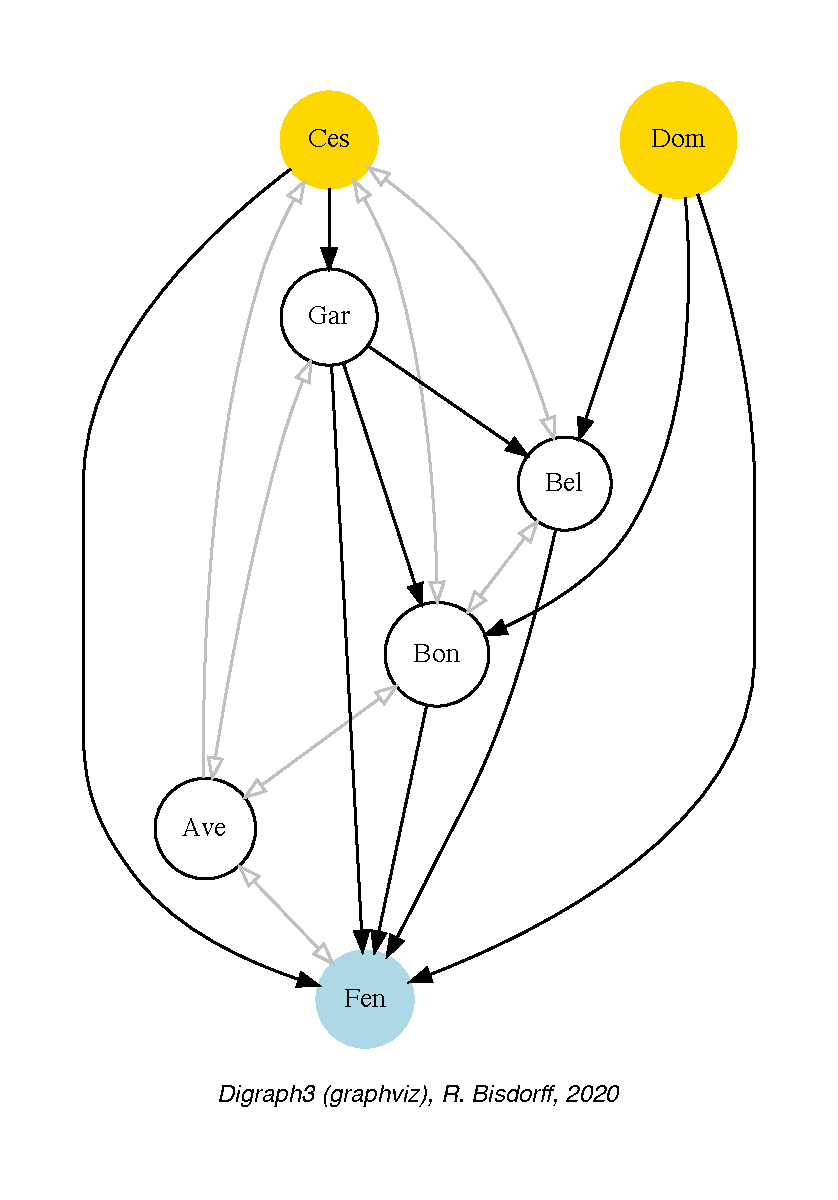
\includegraphics[width=6cm]{Figures/4-3-bestOfficeChoice.pdf}
\caption[Best office choice recommendation from strict outranking digraph]{\emph{Best office choice recommendation from strict outranking digraph}\\ Notice that location \texttt{A} (\emph{Ave}) (the most expensive) is appearing \emph{incomparable} to all the other alternatives.}
\label{fig:4.3}       % Give a unique label
\end{figure}

Let us finally notice in Listing~\vref{list:4.4} Line~\ref{line:4.4.18} that both alternatives \texttt{A} and \texttt{F} are reported as potential last choice recommendation. Yet, this last choice recommendation appears to be globally indeterminate (Lines~\ref{line:4.4.25}--\ref{line:4.4.26}). This confirms the \emph{incomparability} status of alternative \texttt{A} (see Fig.~\vref{fig:4.3}).
\begin{lstlisting}
>>> bodcd.exportGraphViz(fileName='bestOfficeChoice',\
...                    firstChoice=['C','D'],\
...                    lastChoice=['F'])
  *---- exporting a dot file for GraphViz tools ---------*
   Exporting to bestOfficeChoice.dot
   dot -Grankdir=BT -Tpng bestOfficeChoice.dot \
                    -o bestOfficeChoice.png
\end{lstlisting}

\section{Weakly ordering the outranking digraph}
\label{sec:4.6}

To get a global insight in the overall strict outranking situations, we may use the \texttt{RankingByChoosingDigraph}\index{RankingByChoosingDigraph@\texttt{RankingByChoosingDigraph} class} class imported from the \texttt{transitive\-Digraphs}\index{transitiveDigraphs@\texttt{transitiveDigraphs} module} module for computing a \emph{ranking-by-choosing} result from the codual, i.e. the strict outranking digraph instance \texttt{bodcd} (see above). If the computing node supports multiple processor cores, \emph{first} and \emph{last} choosing iterations may be run in parallel (see Line~\ref{line:4.7.4} in List.~\vref{list:4.7}).
\begin{lstlisting}[caption={Ranking-by-choosing the outranking digraph},label=list:4.7]
>>> from transitiveDigraphs import\
...                  RankingByChoosingDigraph
>>> rbc = RankingByChoosingDigraph(bodcd)
 Threading ... # multiprocessing if 2 cores are available §\label{line:4.7.4}§
 Exiting computing threads
>>> rbc.showRankingByChoosing()
 Ranking by Choosing and Rejecting
    1st ranked ['D']
       2nd ranked ['C', 'G']
       2nd last ranked ['B', 'C', 'E']
    1st last ranked ['A', 'F']
>>> rbc.exportGraphViz('officeChoiceRanking')
 *---- exporting a dot file for GraphViz tools ---------*
  Exporting to officeChoiceRanking.dot
  dot -Grankdir=TB -Tpng officeChoiceRanking.dot\
                   -o officeChoiceRanking.png
\end{lstlisting}
\begin{figure}[ht]
\sidecaption[t]
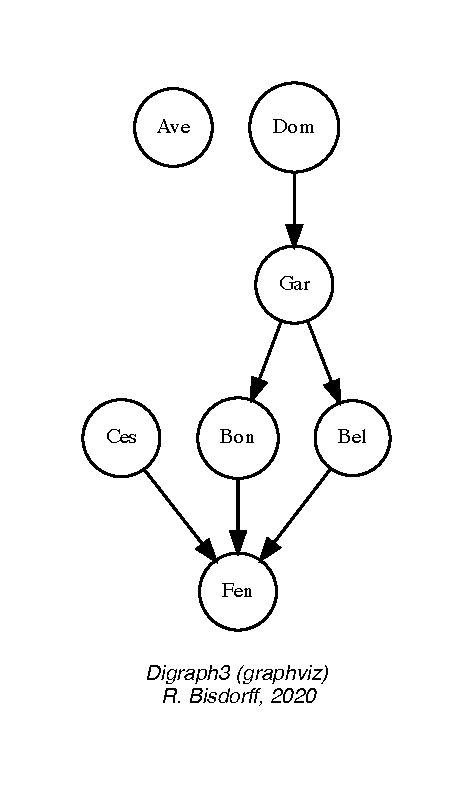
\includegraphics[width=5cm]{Figures/4-4-officeChoiceRanking.pdf}
\caption[Ranking-by-choosing the potential office locations]{\emph{Ranking-by-choosing the potentail office locations}\\ In this \emph{ranking-by-choosing} method, where we operate the \emph{epistemic fusion} of iterated (strict) first and last choices, compromise alternative \texttt{Dom} is now ranked before compromise alternative \texttt{Gar}. The overall partial ordering result shows again the important fact that the most expensive location \texttt{Ave}, and the cheapest location \texttt{Ces}, due to their contradictory performances, appear both \emph{incomparable} with most of the other alternatives.} 
\label{fig:4.4}       % Give a unique label
\end{figure}

The best choice recommendation hence depends on the very importance the CEO is attaching to each of his decision objectives. In the given setting here, where he considers that \emph{maximising the future turnover} is the most important objective followed by \emph{minimising the Costs} and, less important, \emph{maximising the working conditions}, location \texttt{D} represents actually the \emph{best compromise}. However, if \emph{Costs} do not play much a role, it would be perhaps better to decide to move to the most advantageous location \texttt{A}; or if, on the contrary, \emph{Costs} do matter a lot, moving to the cheapest alternative \texttt{C} could definitely represent a more convincing recommendation. 

It might be worth editing the criteria significance weights in the\\
\texttt{officeChoice.py} data file in such a way that:
\begin{itemize}[topsep=2pt]
\item All three decision objectives are considered \emph{equally important}, and
\item All criteria under each objective are considered \emph{equi-significant}.
\end{itemize}

What will become the best choice recommendation under this working hypothesis?\footnote{See also the notes of Lecture 7 from the MICS Algorithmic Decision Theory course \citep{ADT-L7}.} 

%\vspace{1cm}
\vspace{\baselineskip}
In the next Chap.~\ref{sec:5} we precisely show how to edit a new performance tableau from a given template file. 

%%%%%%%%%%%%%%%%%%%%%%%%%%%%%%%%%%%%
\phantomsection
\addcontentsline{toc}{section}{Notes}
\section*{Notes}

Following a seminar presentation in 2005 at the LAMSADE\footnote{Laboratoires d'Analyse et de Modélisation de Systèmes d'Aide à la Décision, Université Paris-Dauphine, UMR 7243 CNRS}, where the author promoted the use of kernels of the outranking digraph as suitable candidates for delivering best choice recommendations \citep{BIS-2005}, a critical discussion started about the methodological requirement for a convincing best choice recommendation to be internally stable (pragmatic principle \texttt{P3}). \emph{Denis Bouyssou}\index{Bouyssou@\emph{D. Bouyssou}} illustrated his doubts with the potential outranking digraph shown in Fig.~\vref{fig:4.5}.
\begin{figure}[ht]
\sidecaption[t]
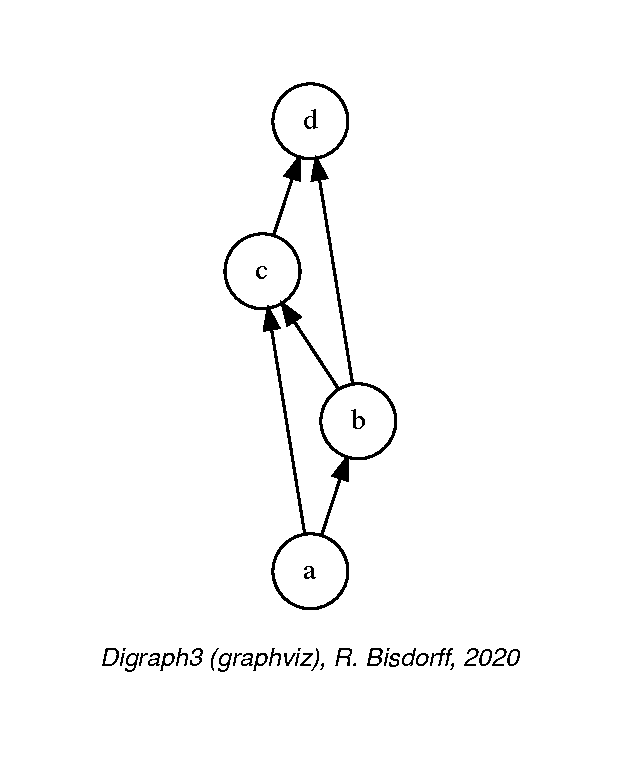
\includegraphics[width=6cm]{Figures/4-5-bouyssou11Oct05crisp.pdf}
\caption[The internal stability of a best choice recommendation in question]{\emph{The internal stability of a best choice recommendation in question}\\ The only kernel of this digraph is the pair $\{\mathtt{a},\mathtt{d}\}$; yet, it is an ambiguous recommendation, as $\{\mathtt{a},\mathtt{d}\}$ is conjointly an outranking and outranked choice. If the instability of the best choice recommendation is, however, not considered a problem then the choice $\{\mathtt{a},\mathtt{b}\}$ shows the most convincing strict outranking quality and could be considered in priority for recommendation as potential best choice candidates.}
\label{fig:4.5}       % Give a unique label
\end{figure}

His commentary was the following: Adding alternative \texttt{d} to the set of potential best choice candidates is not convincing as there exists in the given digraph the node \texttt{b}, which is better evaluated than \texttt{d}. The argument that the incomparability between \texttt{a} and \texttt{d} should favour \texttt{d} as potential best choice is interesting but another hypothesis could be that \texttt{b} perhaps outranks \texttt{a}. In this latter case, it seams clear that the actual best choice recommendation should be reduced to node \texttt{b}, unless one disposes of other information, like a performance tableau and/or the actual computation method of the outranking situations. In any case, one has to be very clear about the available information when judging a best choice procedure.

It became thereafter obvious for us all that both the lack of a specific performance tableau as well as the lack of a precisely defined algorithm for computing valid outranking situations do not allow to judge if a given digraph does indeed model a potential outranking relation. In our present bipolar-valued epistemic approach, a valid outranking digraph instance, following from a given performance tableau and the disjunctive epistemic fusion construction of the outranking relation (see Chap.~\ref{sec:3}), will necessarily verify the weak completeness condition and the coduality principle. As a consequence, incomparability situations are now modelled by epistemic indeterminateness not by the actual absence of a reciprocal outranking relation.

The digraph put forward by \emph{D. Bouyssou} in the October 2005 discussion is not weakly complete --node \texttt{a} is not outranking node \texttt{d} and vice versa-- and does hence not represent, in our present sense, a valid outranking digraph instance. Yet, it may be a partial tournament and as such it could be a strict outranking digraph, i.e. the asymmetric part --the codual-- of a valid outranking digraph. In this case, nodes \texttt{a} and \texttt{d} --the kernel of the strict outranking digraph-- would actually for sure outrank each other and, hence, represent both indifferently the natural best choice recommendation. However, in this not strict codual digraph, node \texttt{a} becomes also the unique \Condorcet winner --outranking for sure all other nodes-- and gives hence the evident unique best choice recommendation.

Only after 2013, when the weak completeness and the coduality properties of the outranking digraph were discovered, became it obvious that the initial prekernels of the strict outranking digraph, coupled with the solution of the corresponding kernel equation system, were in fact delivering the most convincing best choice recommendations (see Chap.~\ref{sec:17}, Sect.~\ref{sec:20.4} and \citealp{BIS-2013}). It stays an interesting open mathematical problem to show (or not) that both necessary conditions: --weak completeness and coduality-- are also sufficient for qualifying any bipolar-valued digraph as potential instance of an outranking digraph.


%%%%%%% The chapter bibliography
%\normallatexbib
%\clearpage
%\phantomsection
%\addcontentsline{toc}{section}{Chapter Bibliography}
\chapter{Building a best choice recommendation}
\label{sec:4}

\abstract*{  This chapter presents the \Rubis best choice recommender system. Our approach is illustrated with building a best office site recommendation. We show how to explore the given performance tableau and compute the corresponding outranking digraph. After presenting the pragmatic principles that govern our best choice recommendation algorithm we solve the best office-location choice problem.}

\begin{quotation}
  ``... \emph{The goal of our research was to design a resolution method} ... \emph{that is easy to put into practice, that requires as few and reliable hypotheses as possible, and that meets the needs} [of the decision maker]...''

  --\citep*{ROY-1966}\index{Roy@\textsl{B. Roy}}.
\end{quotation}
\vspace{1cm}

\abstract{ This chapter presents the \Rubis best choice recommender system. Our approach is illustrated with a best office location selection problem. We show how to explore the given performance tableau and compute the corresponding outranking digraph. After presenting the pragmatic principles that govern our best choice recommendation algorithm we solve the best office location choice problem.}

\section{What office-location to choose?}
\label{sec:4.1}

A SME, specialised in printing and copy services, has to move into new offices, and its CEO has gathered seven \emph{potential new office locations} (see Table~\vref{tab:4.1}).
\begin{table}[ht]
\caption{The potential new office locations}
\label{tab:4.1}       % Give a unique label
\begin{center}
  %\begin{small}
    \begin{tabular}{c|l|l|l}
      \svhline\noalign{\smallskip}
      ID & Name & Address & Comment\\
      \noalign{\smallskip}\hline\noalign{\smallskip}
    A &   Ave  &  Avenue de la liberté &  High standing city center\\
    B &   Bon  &  Bonnevoie &             Industrial environment\\
    C &   Ces  &  Cessange &              Residential suburb location\\
    D &   Dom  &  Dommeldange &           Industrial suburb environment\\
    E &   Bel  &  Esch-Belval &           New and ambitious urbanisation far from the city\\
    F &   Fen  &  Fentange &              Out in the countryside\\
      G &   Gar  &  Avenue de la Gare &     Main city shopping street\\
      \noalign{\smallskip}\hline
    \end{tabular}
  %\end{small}
\end{center}
\end{table}

Three \emph{decision objectives}, in order of decreasing importance, are guiding the CEO's choice:
\begin{enumerate}[leftmargin=1cm]
\item \emph{maximise} the future turnover of the SME,
\item \emph{minimise} the future yearly costs induced by the moving,
\item \emph{maximise} the new working conditions.
\end{enumerate}

The decision consequences to take into account for evaluating the potential new office locations with respect to each one of the three objectives are modelled by the \emph{family of performance criteria} \footnote{See \citealp{ROY-2000}} shown in Table~\vref{tab:4.2} below.
\begin{table}[ht]
\caption{The family of performance criteria}
\label{tab:4.2}       % Give a unique label
\begin{center}
    \begin{tabular}{l|c|c|c|l}
      \svhline\noalign{\smallskip}
      Objective & ID & Name & Weight & Comment\\
      \noalign{\smallskip}\hline\noalign{\smallskip}
    Yearly costs  &       Ct &   Costs &  45 &     Annual rent, charges, and cleaning\\
    \             &  \      & \        &  \ & \ \\
    Future turnover   &   Pr  & Proximity  & 32 & Distance from town center\\
    Future turnover   &   V  &  Visibility & 26 & Circulation of potential customers \\
    Future turnover   &   St &   Standing & 23 &   Image and presentation\\
    \                 &   \   & \          &  \ & \  \\
    Working conditions &  W  &  Space   &   10 &  Working space\\
    Working conditions &  Cf &  Comfort  &  6 &  Quality of office equipment\\
    Working conditions &  P  &  Parking  &  3 &  Available parking facilities\\
      \noalign{\smallskip}\hline
    \end{tabular}   
  \end{center}
\end{table}

In Table~\vref{tab:4.2} we notice that the \emph{Costs} criterion admits the highest significance weight ($45$), followed by the \emph{Future turnover} criteria $(32, 26, 23)$, The \emph{Working conditions} criteria are the less significant $(10, 6, 3)$ \footnote{These criteria weights were supposedly established with a swing weighing MCDA method \citep{KEE-1976}.}. It follows that the CEO considers \emph{maximising the future turnover} the most important objective ($(32 + 26+ 23) = 81$), followed by minimising the future yearly costs ($45$), and less important, \emph{maximising working conditions} ($(10 + 6 + 3) = 19$). 

The evaluations of the seven potential new locations on each performance criterion are gathered in a \emph{performance table} shown in Table~\vref{tab:4.3}.
\begin{table}[ht]
\caption{Performance evaluations of the potential office locations}
\label{tab:4.3}       % Give a unique label
\begin{center}
    \begin{tabular}{l|c|c|c|c|c|c|c}
      \svhline\noalign{\smallskip}
    Criterion  &    A  &      B &       C &       D &       E &        F &        G\\
       \noalign{\smallskip}\hline\noalign{\smallskip}

    Costs      &   35.0K€ &  17.8K€  & 6.7K€  &  14.1K€ &  34.8K€ &  18.6K€ &  12.0K€\\
    \          &   \      &  \     &   \     &   \    &    \    &    \    &    \ \\
    Proximity     &   100    &  20 &      80    &   70    &   40    &   0    &    60 \\
    Visibility     &   60     &  80  &     70    &   50    &   60    &   0    &    100 \\
    Standing      &   100   &   10   &    0     &   30    &   90    &   70   &    20 \\
    \           &   \     &   \    &    \     &   \     &   \     &   \    &    \  \\
    Working space      &   75    &   30   &    0     &   55    &   100   &   0    &    50  \\
    Working comfort      &   0     &   100  &    10    &   30    &   60    &   80   &    50 \\
    Parking     &   90    &   30   &    100   &   90    &   70    &   0    &    80 \\
      \noalign{\smallskip}\hline
    \end{tabular}
  \end{center}
\end{table}
All criteria, except the \emph{Costs} Criterion, admit for evaluation a qualitative satisfaction scale from $0\%$ (weakest) to $100\%$ (highest). One may thus notice that location \texttt{A} (\emph{Ave}) is the most expensive, but also $100\%$ satisfying the \emph{Proximity} as well as the  \emph{Standing} criterion. Whereas location \texttt{C} (\emph{Ces}) is the cheapest one; providing however no satisfaction at all on both the \emph{Standing} and the \emph{Working Space} criteria.

Concerning yearly costs, we suppose that the CEO is indifferent up to a performance difference of $1000.00$€, and he actually prefers a location when there is at least a positive difference of $2500.00$€. The evaluations observed on the six qualitative criteria (measured in percentages of satisfaction) are very subjective and rather imprecise. The CEO is hence \emph{indifferent} up to a satisfaction difference of $10\%$, and he claims a significant \emph{preference} when the satisfaction difference is at least of $20\%$.  Furthermore, a satisfaction difference of $80\%$ represents for him a \emph{considerably large} performance difference, triggering the case given a \emph{polarisation} of the preferential situation \citep{BIS-2013}. 

In view of Table~\vref{tab:4.3}, what is now the office location we may recommend to the CEO as \textbf{best choice}?

\section{The given performance tableau}
\label{sec:4.2}


The file \texttt{officeChoice.py}, stored in the \texttt{examples} directory of the \Digraph resources, provides a corresponding \texttt{PerformanceTableau}\index{PerformanceTableau@\texttt{PerformanceTableau} class} object. We can inspect its actual content with the computing resources provided by the \texttt{perfTabs} module \index{perfTabs@\texttt{perfTabs} module}.
\begin{lstlisting}[caption={Inspecting the \texttt{officeChoice} performance tableau.},label=list:4.1]
>>> from perfTabs import PerformanceTableau
>>> pt = PerformanceTableau('officeChoice')
>>> pt
 *------- PerformanceTableau instance description ------*
   Instance class     : PerformanceTableau
   Instance name      : officeChoice
   Actions            : 7
   Objectives         : 3
   Criteria           : 7
   NaN proportion (%) : 0.0
   Attributes         : ['name', 'actions', 'objectives',
                         'criteria', 'weightPreorder',
			 'NA', 'evaluation']
>>> pt.showPerformanceTableau()
 *----  performance tableau -----*
  Criteria|  'Ct'       'Cf'   'P'   'Pr'   'St'    'V'    'W'   
  Weights |  45.00      6.00   3.00  32.00  23.00  26.00  10.00    
  --------|----------------------------------------------------
   'Ave'  | -35000.00   0.00  90.00 100.00 100.00  60.00  75.00  
   'Bon'  | -17800.00 100.00  30.00  20.00  10.00  80.00  30.00  
   'Ces'  |  -6700.00  10.00 100.00  80.00   0.00  70.00   0.00  
   'Dom'  | -14100.00  30.00  90.00  70.00  30.00  50.00  55.00  
   'Bel'  | -34800.00  60.00  70.00  40.00  90.00  60.00 100.00  
   'Fen'  | -18600.00  80.00   0.00   0.00  70.00   0.00   0.00  
   'Gar'  | -12000.00  50.00  80.00  60.00  20.00 100.00  50.00  
\end{lstlisting}

We thus recover all the input data shown in Section~\ref{sec:4.1}. Notice that the \emph{negative} evaluations of the \emph{Costs} criterion indicate a negative preference direction: the \emph{lower} the costs, the \emph{better} it is.

The \texttt{showCriteria()}\index{showCriteria@\texttt{showCriteria()}} method evaluates the actual preference discrimination we observe on each performance criterion.
\begin{lstlisting}[caption={Inspecting the performance criteria.},label=list:4.2]
>>> pt.showCriteria(IntegerWeights=True)
 *----  criteria -----*
  Ct 'Costs'
   Preference direction: min
   Scale = (0.00, 50000.00)
   Weight = 45
   Threshold ind : 1000.00 + 0.00x ;  percentile:  9.52 §\label{line:4.2.7}§
   Threshold pref : 2500.00 + 0.00x ; percentile: 14.29 §\label{line:4.2.8}§
  Cf 'Comfort'
   Preference direction: max
   Scale = (0.00, 100.00)
   Weight = 6
   Threshold ind : 10.00 + 0.00x ;  percentile:   9.52 §\label{line:4.2.13}§
   Threshold pref : 20.00 + 0.00x ; percentile:  28.57 §\label{line:4.2.14}§
   Threshold veto : 80.00 + 0.00x ; percentile:  90.48 §\label{line:4.2.15}§
   ...
   ...
\end{lstlisting}

On the \emph{Costs} criterion, $9.5\%$ of the performance differences are considered insignificant and $14.3\%$ below the preference discrimination threshold (see Lines~\ref{line:4.2.7}--\ref{line:4.2.8} in List.~\vref{list:4.2}). On the qualitative \emph{Comfort} criterion, we observe again $9.5\%$ of insignificant performance differences (line~\ref{line:4.2.13}). Due to the imprecision in the subjective evaluations, we notice here $28.6\%$ of performance differences below the preference discrimination threshold (Line~\ref{line:4.2.14}). Furthermore, $100.0 - 90.5 = 9.5\%$ of the performance differences are judged \emph{considerably large} (Line~\ref{line:4.2.15}) and will trigger hence a polarisation of the concerned outranking situations \citep{BIS-2013}. Same information is available for all the other criteria. 
 
A colourful comparison of all the evaluations is shown in Fig.~\vref{fig:4.1} by the \emph{heatmap}\index{showHTMLPerformanceHeatmap@\texttt{showHTMLPerformanceHeatmap()}} statistics, illustrating the respective quantile class of each evaluation. As the set of potential alternatives is tiny, we choose here a classification into performance quintiles.
\begin{lstlisting}
>>> pt.showHTMLPerformanceHeatmap(colorLevels=5,\
...                              rankingRule=None)
\end{lstlisting}
    \begin{figure}[ht]
%\sidecaption
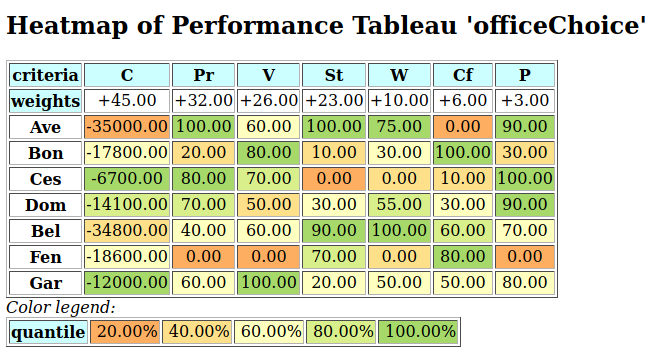
\includegraphics[width=0.8\hsize]{Figures/4-1-officeChoiceHeatmap.png}
\caption{Unranked heatmap of the office choice performance tableau}
\label{fig:4.1}       % Give a unique label
\end{figure}

Location \texttt{Ave} shows extreme and contradictory evaluations: highest \emph{Costs} and no \emph{Working Comfort} on the one hand, and total satisfaction with respect to \emph{Standing}, \emph{Proximity} and \emph{Parking facilities} on the other hand. Similar, but opposite, situation is given for location \texttt{Ces}: unsatisfactory \emph{Working Space}, no \emph{Standing} and no \emph{Working Comfort} on the one hand, and lowest \emph{Costs}, best \emph{Proximity} and \emph{Parking facilities} on the other hand. Contrary to these contradictory alternatives, we observe two appealing compromise alternatives: locations \texttt{Dom} and \texttt{Gar}. Finally, location \texttt{Fen} is clearly the less satisfactory alternative of all.

To help now the CEO choosing the best office location, we are going to compute pairwise outranking situations on the set of potential decision alternatives (see \citealp{BIS-2013}).

\section{Computing the outranking digraph}
\label{sec:4.3}

\begin{definition}[Outranking situation]\label{def:outranking}\index{outranking!situation}

\noindent For two potential decision alternatives $x$ and $y$:
\begin{itemize}[leftmargin=0.5cm,rightmargin=0.5cm]
\item ``Alternative $x$ \emph{outranks} alternative $y$'', denoted $(x \succsim y)$, is given when:
   \begin{enumerate}[nosep]
     \item A \emph{majority} of criteria significance warrants that alternative $x$ is \emph{at least as well evaluated as} alternative $y$, and
     \item \emph{No considerable} negative performance difference is observed on any criterion.      
    \end{enumerate}
\item ``Alternative $x$ \emph{does not outrank} $y$'', denoted $(x \not\succsim y)$, is given when:
   \begin{enumerate}[nosep]
    \item Only a \emph{minority} of criteria significance warrants that alternative $x$ is \emph{at least as well evaluated as} alternative $y$, and
    \item \emph{No considerable} positive performance difference is observed on any criterion. 
    \end{enumerate}
\item Otherwise, the outranking situation between alternatives $x$ and $y$ is considered to be \emph{indeterminate}.
\end{itemize}
\end{definition}

The credibility of each pairwise outranking situation, denoted $r(x \succsim y)$, is measured in a bipolar significance valuation $[-1.0, 1.0]$, where \emph{positive} terms $r(x \succsim y)\, >\, 0.0$ indicate a \emph{validated outranking}, and \emph{negative} terms $r(x \succsim y)\, <\, 0.0$ indicate an \emph{invalidated outranking}, i.e. a \emph{validated outranked} situation. The \emph{median} value $r(x \succsim y)\, = \,0.0$ represents an \emph{indeterminate} situation (see \citealp{BIS-2004a} and \citealp{BIS-2013}).   

For computing such a bipolar-valued binary outranking relation from the given performance tableau \texttt{pt}, we use the \texttt{BipolarOutrankingDigraph}\index{BipolarOutrankingDigraph@\texttt{BipolarOutrankingDigraph} class} class from the \texttt{outrankingDigraphs}\index{outrankingDigraphs@\texttt{outrankingDigraphs} module} module. The corresponding
\texttt{showHTMLRe\-lation\-Table()}\index{showHTMLRelationTable@\texttt{showHTMLRelationTable()}} method shows here the resulting bipolar-valued adjacency matrix in a system browser window (see Fig.~\vref{fig:4.2}).
\begin{lstlisting}[caption={Computing a bipolar-valued outranking digraph},label=list:4.3]
>>> from outrankingDigraphs import BipolarOutrankingDigraph
>>> bod = BipolarOutrankingDigraph(pt)
>>> bod.showHTMLRelationTable()
\end{lstlisting}
\begin{figure}[ht]
\sidecaption[t]
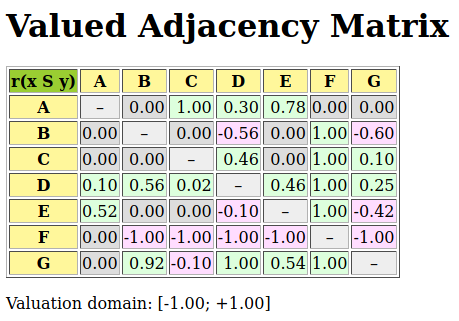
\includegraphics[width=7cm]{Figures/4-2-officeChoiceOutranking.png}
\caption[Bipolar-valued adjacency matrix]{\emph{Bipolar-valued adjacency matrix}\\ In the resulting outranking relation we may notice, on the one hand, that Alternative \texttt{D} is \emph{positively outranking} all other potential office locations. On the other hand, alternatives \texttt{A} (the most expensive) and \texttt{C} (the cheapest) are \emph{not outranked} by any other location.}
\label{fig:4.2}       % Give a unique label
\end{figure}

Alternative \texttt{D} gives a \Condorcet winner\footnote{See Chap.~\ref{sec:7} on computing the winner of an election.}, whereas alternatives \texttt{A} (the most expensive) and \texttt{C} (the cheapest) give in fact \emph{weak} \Condorcet winners.\index{computeCondorcetWinners@\texttt{computeCondorcetWinners()}}\index{computeWeakCondorcetWinners@\texttt{computeWeakCondorcetWinners()}}
\begin{lstlisting}
>>> bod.computeCondorcetWinners()
 ['D']
>>> bod.computeWeakCondorcetWinners()
 ['A', 'C', 'D']
\end{lstlisting}

From theory, we know that outranking digraphs are \emph{weakly complete}\index{weakly complete}, i.e. for all $x$ and $y$ in $X$, $r(x \succsim y)\, <\, 0.0$ implies that $r(y \succsim x)\, \geqslant \, 0.0$. And, they verify the \emph{coduality principle}\index{coduality principle}:  $r(x \not\succsim y) \; = \; r(y \succnsim x)$ \citep{BIS-2013}.\footnote{Not to be confused with the dual graph of a plane graph \texttt{g} that has a vertex for each face of \texttt{g}. Here we mean the \emph{less than} (strict converse) relation corresponding to a \emph{greater or equal} relation, or the \emph{less than or equal} relation corresponding to a (strict) \emph{better than} relation.}

\begin{definition}[Strict outranking situation]\label{def:strictOutranking}\index{outranking!strict situation}

\noindent For two potential decision alternatives $x$ and $y$, ``$x$ \emph{strictly outranks} alternative $y$'', denoted $(x \succnsim y)$, when ``$x$ \emph{outranks} alternative $y$'' ($(x \succsim y) > 0.0$) and ``$y$ \emph{does not outrank} alternative $x$'' ($(y \succsim x) < 0.0$).
\end{definition}

Following from the coduality principle, the strict outranking digraph \texttt{bodcd} is build from the outranking digraph \texttt{bod} with a codual transform\index{codual transform} (see Sect.~\ref{sec:2.6}).
\begin{lstlisting} 
>>> bodcd = ~(-bod)  # codual tranform
>>> bodcd
*------- Object instance description ------*
Instance class       : BipolarOutrankingDigraph
Instance name        : converse-dual-rel_officeChoice
Actions              : 7
Criteria             : 7
Size                 : 10
Determinateness (%)  : 72.38
Valuation domain     : [-1.00;1.00]
\end{lstlisting}


\section{Designing a best choice recommender system}
\label{sec:4.4}

Solving a best-choice problem consists traditionally in finding \emph{the} unique best decision alternative. We adopt here instead a modern recommender system’s approach which shows a non empty subset of decision alternatives which contains by construction the potential best alternative(s).

The five \emph{pragmatic principles} for computing such a \emph{best-choice recommendation} (BCR) are the following:
\begin{itemize}[leftmargin=1cm,listparindent=0em]
\item [\texttt{P1}:] \emph{Elimination for well motivated reasons}; each eliminated alternative has to be strictly outranked by at least one alternative in the BCR.
\item [\texttt{P2}:] \emph{Minimal size}; the BCR must be as limited in cardinality as possible.
\item [\texttt{P3}:] \emph{Efficient and informative}; The BCR must not contain a self-contained sub-recommendation.
\item [\texttt{P4}:] \emph{Effectively better}; the BCR must not be ambiguous in the sense that it may not be both a first choice as well as a last choice recommendation.
\item [\texttt{P5}:] \emph{Maximally determined}; the BCR is, of all potential best-choice recommendations, the most determined one in the sense of the epistemic characteristics of the bipolar-valued outranking relation.
\end{itemize}

Let $X$ be the set of potential decision alternatives. Let $Y$ be a non empty subset of $X$, called a \emph{choice} in the strict outranking digraph $G(X,r(\succnsim )$. We can now qualify a BCR $Y$ in following terms:
\begin{itemize}[leftmargin=0.5cm,listparindent=0em]
\item [-] $Y$ is called strictly \emph{outranking} (resp. \emph{outranked}) when for all not selected alternative $x$ there exists an alternative $y \in X$ retained such that $r(y \succnsim x) > 0.0$ (resp. $r(y \precsim x) > 0.0$). Such a choice verifies principle \texttt{P1}.
\item [-] $Y$ is called \emph{weakly independent} when for all $x \neq y$ in $Y$ we observe $r(x \succnsim y) \leq 0.0$. Such a choice verifies principles \texttt{P3} (\emph{internal stability}).
\item [-] $Y$ is conjointly a strictly \emph{outranking} (resp. \emph{outranked}) \textbf{and} \emph{weakly independent} choice. Such a choice is called an \emph{initial} (resp. \emph{terminal}) \emph{prekernel}\footnote{See Chap.~\ref{sec:17} on computing kernels in digraphs}. The initial prekernel now verifies principles \texttt{P1}, \texttt{P2}, \texttt{P3} and \texttt{P4}. 
\item [-] To finally verify principle \texttt{P5}, we recommend among all potential initial prekernels, a \emph{most determined} one, i.e. a strictly \emph{outranking} and \emph{weakly independent} choice supported by the highest criteria significance. And in this most determined initial prekernel we eventually retain the alternative(s) that are included with highest criteria significance\footnote{See Sect.~\ref{sec:17.6}}.
\end{itemize}

Mind that a given strict outranking digraph may not always admit prekernels. This is the case when the digraph contains chordless circuits of odd length (see Chap.~\ref{sec:17}). Luckily, our strict outranking digraph \texttt{bodcd} here does not show any chordless outranking circuits; a fact we can check with the \texttt{computeChordless\-Cir\-cuits()} method\index{computeChordlessCircuits@\texttt{computeChordlessCircuits()}} followed by the \texttt{showChordlessCircuits()} method\index{showChordlessCircuits@\texttt{showChordlessCircuits()}}\footnote{The \texttt{computeChordlessCircuits()} and \texttt{showChordlessCircuits()} methods are separate because there are various methods available for enumerating the chordless circuits in a digraph \citep{BIS-2010}.}.
\begin{lstlisting}
>>> bodcd.computeChordlessCircuits()
  []  
>>> bodcd.showChordlessCircuits()
  No circuits observed in this digraph.
\end{lstlisting}

When observing chordless odd outranking circuits, we need to break them open with the \texttt{BrokenCocsDigraph} class at their weakest link, before enumerating the prekernels. \citep{BIS-2021b}.\index{BrokenCocsDigraph@\texttt{BrokenCocsDigraph} class}

We are ready now for building a best best choice recommendation.

\section{Computing the \Rubis best choice recommendation}
\label{sec:4.5}

The \texttt{showBestChoiceRecommendation()} method\index{showBestChoiceRecommendation@\texttt{showBestChoiceRecommendation()}} computes the \Rubis best choice recommendation directly from the outranking digraph $bod$. By default this method is operating on the \emph{codual} (strict) outranking digraph where chordless odd circuits have been bropen up (see the \texttt{CoDual} and \texttt{BrokenCocs} parameters in List.~\vref{list:4.4} Line~\ref{line:4.4.2}):
\begin{lstlisting}[caption={Computing the best choice recommendation},label=list:4.4]
>>> bod.showBestChoiceRecommendation(\
...              CoDual=True, BrokenCocs=True # default settings\ §\label{line:4.4.2}§
...              ChoiceVector = True)   §\label{line:4.4.3}§
  * --- First and last choice recommendation(s) ---*
    (in decreasing order of determinateness)   
    Credibility domain: [-1.00,1.00]
    === >> potential first choice(s)
    * choice              : ['A', 'C', 'D'] §\label{line:4.4.8}§
      independence        : 0.00
      dominance           : 0.10
      absorbency          : 0.00
      covering (%)        : 41.67
      determinateness (%) : 50.59
      - characteristic vector = {
        'D': +0.02, 'G': 0.00, 'C': 0.00, 'A': 0.00, §\label{line:4.4.15}§
        'F': -0.02, 'E': -0.02, 'B': -0.02, } §\label{line:4.4.16}§
    === >> potential last choice(s) 
    * choice              : ['A', 'F'] §\label{line:4.4.18}§
      independence        : 0.00
      dominance           : -0.52
      absorbency          : 1.00
      covered (%)         : 50.00
      determinateness (%) : 50.00
      - characteristic vector = {
        'G': 0.00, 'F': 0.00, 'E': 0.00, 'D': 0.00, §\label{line:4.4.25}§
        'C': 0.00, 'B': 0.00, 'A': 0.00, }          §\label{line:4.4.26}§
\end{lstlisting}				  

It is interesting to notice in Line~\ref{line:4.4.8} above that the \Rubis \emph{first choice recommendation} consists actually in the previously mentioned set of weak \Condorcet winners\index{Condorcet@\Condorcet!winner}: \texttt{A}, \texttt{C} and \texttt{D} (see Fig.~\vref{fig:4.2}). In the corresponding prekernel characteristic vector (see Lines~\ref{line:4.4.3},~\ref{line:4.4.15} and Sect.~\ref{sec:17.6}), representing the bipolar credibility degree with which each alternative may indeed be included in, or excluded from this recommendation, we find that alternative \texttt{D} is the only positively validated one, whereas both extreme alternatives --\texttt{A} (the most expensive) and \texttt{C} (the cheapest)-- stay in an indeterminate situation (see \citealp{BIS-2006a,BIS-2006b}). They may \emph{be or not be} potential best choices. Notice furthermore that compromise alternative \texttt{G}, while not actually being included in this strictly outranking prekernel, shows as well an indeterminate situation with respect to \emph{being or not being} recommended as potential best choice. Alternatives \texttt{B}, \texttt{E} and \texttt{F} are all negatively included, i.e. positively excluded, from this best choice recommendation (see Line~\ref{line:4.4.16}).

To inspect why alternative \texttt{D} is the only positive best choice recommendation, we shall compare now the evaluations of alternatives \texttt{D} and \texttt{G} in a pairwise perspective\index{showPairwiseComparison@\texttt{showPairwiseComparison()}}.
\begin{lstlisting}[caption={Inspecting pairwise comparison between alternatives \texttt{G} and \texttt{D}},label=list:4.5,basicstyle=\ttfamily\scriptsize]
>>> bod.showPairwiseComparison('G','D')
 *------------  pairwise comparison ----*
  Comparing actions : ('G', 'D')
  crit.  wght.    g(x)      g(y)    diff.  |   ind.    pref.  concord. 
  ====================================================================
   Costs 45.00 -12000.00 -14100.00 +2100.00 | 1000.00 2500.00  +45.00  
   Comf.  6.00     50.00     30.00   +20.00 |   10.00   20.00   +6.00 
   Park.  3.00     80.00     90.00   -10.00 |   10.00   20.00   +3.00 
   Prox. 32.00     60.00     70.00   -10.00 |   10.00   20.00  +32.00 
   Stdg. 23.00     20.00     30.00   -10.00 |   10.00   20.00  +23.00 
   Visi. 26.00    100.00     50.00   +50.00 |   10.00   20.00  +26.00 
   Spac. 10.00     50.00     55.00    -5.00 |   10.00   20.00  +10.00
   =====================================================================
    Valuation in range: -145.00 to +145.00; global concordance: +145.00
\end{lstlisting}

In Listing~\vref{list:4.5}, we notice that, with the given preference discrimination thresholds, alternative \texttt{G} is actually \emph{certainly at least as well evaluated as} alternative \texttt{D}:  $r(G \succsim D)\, = \, +145/145\, =\, +1.0$.

Yet, we must as well acknowledge in Listing~\vref{list:4.6}, that the cheapest alternative \texttt{C} is in fact \emph{strictly outranking} alternative \texttt{G}:  $r(C \succsim G)\, =\, +15/145\, >\, 0.0$, and $r(G \succsim C)\, =\, -15/145 \,<\, 0.0$.
\begin{lstlisting}[caption={Inspecting pairwise comparison between alternatives \texttt{C} and \texttt{G}},label=list:4.6,basicstyle=\ttfamily\scriptsize]
>>> bod.showPairwiseComparison('C','G')
 *------------  pairwise comparison ----*
  Comparing actions : (C,G)/(G,C)
  crit. wght.   g(x)     g(y)      diff.  |   ind.   pref.       (C,G)/(G,C)
   ==========================================================================
   'C'   45.00 -6700.00 -12000.00 +5300.00 | 1000.00 2500.00    +45.00/-45.00 
   'Cf'   6.00    10.00     50.00   -40.00 |   10.00   20.00     -6.00/ +6.00 
   'P'    3.00   100.00     80.00   +20.00 |   10.00   20.00     +3.00/ -3.00 
   'Pr'  32.00    80.00     60.00   +20.00 |   10.00   20.00    +32.00/-32.00 
   'St'  23.00     0.00     20.00   -20.00 |   10.00   20.00    -23.00/+23.00 
   'V'   26.00    70.00    100.00   -30.00 |   10.00   20.00    -26.00/+26.00 
   'W'   10.00     0.00     50.00   -50.00 |   10.00   20.00    -10.00/+10.00
                                                               --------------
    Valuation in range: -145 to +145;      r(C >= G)/r(G >= c): +15.00/-15.00
\end{lstlisting}
\begin{figure}[ht]
\sidecaption[t]
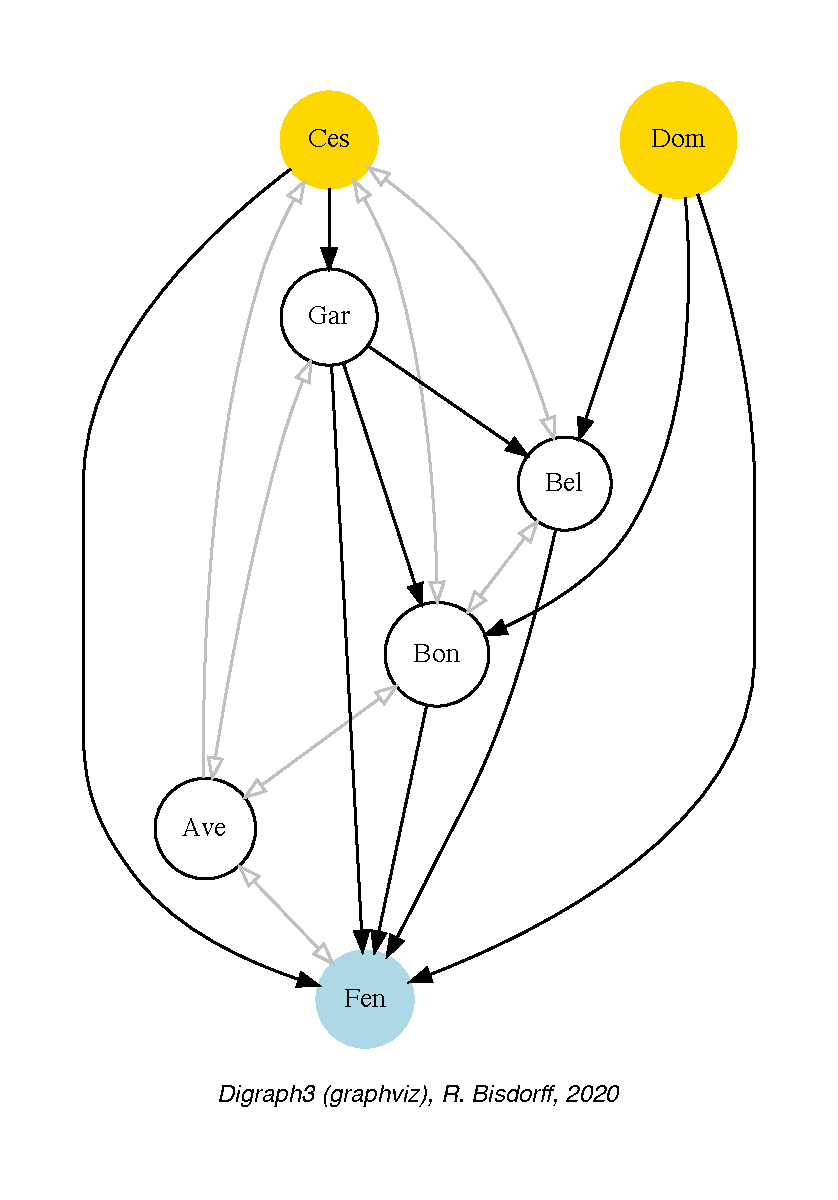
\includegraphics[width=6cm]{Figures/4-3-bestOfficeChoice.pdf}
\caption[Best office choice recommendation from strict outranking digraph]{\emph{Best office choice recommendation from strict outranking digraph}\\ Notice that location \texttt{A} (\emph{Ave}) (the most expensive) is appearing \emph{incomparable} to all the other alternatives.}
\label{fig:4.3}       % Give a unique label
\end{figure}

Let us finally notice in Listing~\vref{list:4.4} Line~\ref{line:4.4.18} that both alternatives \texttt{A} and \texttt{F} are reported as potential last choice recommendation. Yet, this last choice recommendation appears to be globally indeterminate (Lines~\ref{line:4.4.25}--\ref{line:4.4.26}). This confirms the \emph{incomparability} status of alternative \texttt{A} (see Fig.~\vref{fig:4.3}).
\begin{lstlisting}
>>> bodcd.exportGraphViz(fileName='bestOfficeChoice',\
...                    firstChoice=['C','D'],\
...                    lastChoice=['F'])
  *---- exporting a dot file for GraphViz tools ---------*
   Exporting to bestOfficeChoice.dot
   dot -Grankdir=BT -Tpng bestOfficeChoice.dot \
                    -o bestOfficeChoice.png
\end{lstlisting}

\section{Weakly ordering the outranking digraph}
\label{sec:4.6}

To get a global insight in the overall strict outranking situations, we may use the \texttt{RankingByChoosingDigraph}\index{RankingByChoosingDigraph@\texttt{RankingByChoosingDigraph} class} class imported from the \texttt{transitive\-Digraphs}\index{transitiveDigraphs@\texttt{transitiveDigraphs} module} module for computing a \emph{ranking-by-choosing} result from the codual, i.e. the strict outranking digraph instance \texttt{bodcd} (see above). If the computing node supports multiple processor cores, \emph{first} and \emph{last} choosing iterations may be run in parallel (see Line~\ref{line:4.7.4} in List.~\vref{list:4.7}).
\begin{lstlisting}[caption={Ranking-by-choosing the outranking digraph},label=list:4.7]
>>> from transitiveDigraphs import\
...                  RankingByChoosingDigraph
>>> rbc = RankingByChoosingDigraph(bodcd)
 Threading ... # multiprocessing if 2 cores are available §\label{line:4.7.4}§
 Exiting computing threads
>>> rbc.showRankingByChoosing()
 Ranking by Choosing and Rejecting
    1st ranked ['D']
       2nd ranked ['C', 'G']
       2nd last ranked ['B', 'C', 'E']
    1st last ranked ['A', 'F']
>>> rbc.exportGraphViz('officeChoiceRanking')
 *---- exporting a dot file for GraphViz tools ---------*
  Exporting to officeChoiceRanking.dot
  dot -Grankdir=TB -Tpng officeChoiceRanking.dot\
                   -o officeChoiceRanking.png
\end{lstlisting}
\begin{figure}[ht]
\sidecaption[t]
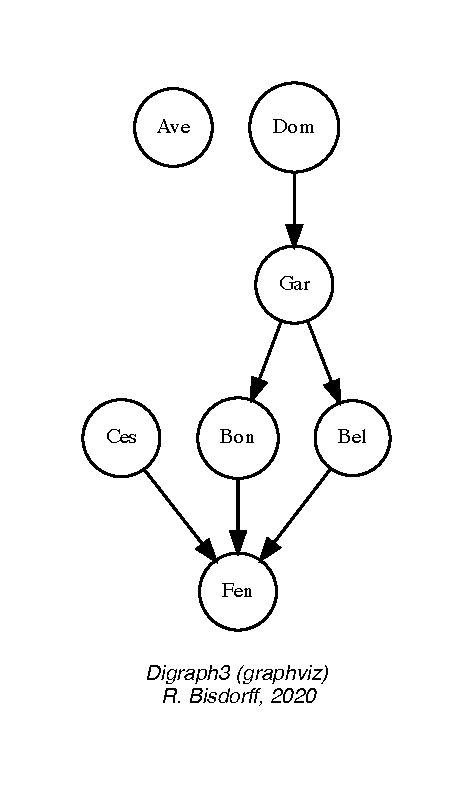
\includegraphics[width=5cm]{Figures/4-4-officeChoiceRanking.pdf}
\caption[Ranking-by-choosing the potential office locations]{\emph{Ranking-by-choosing the potentail office locations}\\ In this \emph{ranking-by-choosing} method, where we operate the \emph{epistemic fusion} of iterated (strict) first and last choices, compromise alternative \texttt{Dom} is now ranked before compromise alternative \texttt{Gar}. The overall partial ordering result shows again the important fact that the most expensive location \texttt{Ave}, and the cheapest location \texttt{Ces}, due to their contradictory performances, appear both \emph{incomparable} with most of the other alternatives.} 
\label{fig:4.4}       % Give a unique label
\end{figure}

The best choice recommendation hence depends on the very importance the CEO is attaching to each of his decision objectives. In the given setting here, where he considers that \emph{maximising the future turnover} is the most important objective followed by \emph{minimising the Costs} and, less important, \emph{maximising the working conditions}, location \texttt{D} represents actually the \emph{best compromise}. However, if \emph{Costs} do not play much a role, it would be perhaps better to decide to move to the most advantageous location \texttt{A}; or if, on the contrary, \emph{Costs} do matter a lot, moving to the cheapest alternative \texttt{C} could definitely represent a more convincing recommendation. 

It might be worth editing the criteria significance weights in the\\
\texttt{officeChoice.py} data file in such a way that:
\begin{itemize}[topsep=2pt]
\item All three decision objectives are considered \emph{equally important}, and
\item All criteria under each objective are considered \emph{equi-significant}.
\end{itemize}

What will become the best choice recommendation under this working hypothesis?\footnote{See also the notes of Lecture 7 from the MICS Algorithmic Decision Theory course \citep{ADT-L7}.} 

%\vspace{1cm}
\vspace{\baselineskip}
In the next Chap.~\ref{sec:5} we precisely show how to edit a new performance tableau from a given template file. 

%%%%%%%%%%%%%%%%%%%%%%%%%%%%%%%%%%%%
\phantomsection
\addcontentsline{toc}{section}{Notes}
\section*{Notes}

Following a seminar presentation in 2005 at the LAMSADE\footnote{Laboratoires d'Analyse et de Modélisation de Systèmes d'Aide à la Décision, Université Paris-Dauphine, UMR 7243 CNRS}, where the author promoted the use of kernels of the outranking digraph as suitable candidates for delivering best choice recommendations \citep{BIS-2005}, a critical discussion started about the methodological requirement for a convincing best choice recommendation to be internally stable (pragmatic principle \texttt{P3}). \emph{Denis Bouyssou}\index{Bouyssou@\emph{D. Bouyssou}} illustrated his doubts with the potential outranking digraph shown in Fig.~\vref{fig:4.5}.
\begin{figure}[ht]
\sidecaption[t]
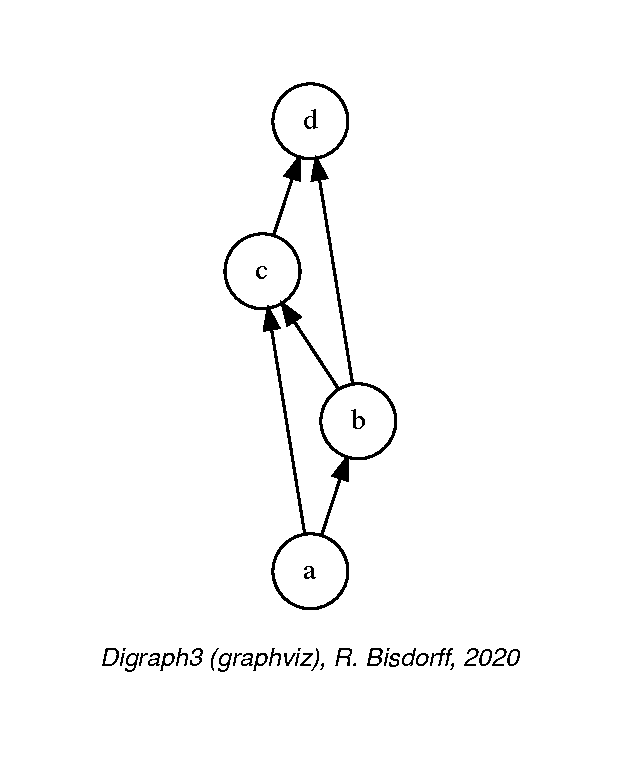
\includegraphics[width=6cm]{Figures/4-5-bouyssou11Oct05crisp.pdf}
\caption[The internal stability of a best choice recommendation in question]{\emph{The internal stability of a best choice recommendation in question}\\ The only kernel of this digraph is the pair $\{\mathtt{a},\mathtt{d}\}$; yet, it is an ambiguous recommendation, as $\{\mathtt{a},\mathtt{d}\}$ is conjointly an outranking and outranked choice. If the instability of the best choice recommendation is, however, not considered a problem then the choice $\{\mathtt{a},\mathtt{b}\}$ shows the most convincing strict outranking quality and could be considered in priority for recommendation as potential best choice candidates.}
\label{fig:4.5}       % Give a unique label
\end{figure}

His commentary was the following: Adding alternative \texttt{d} to the set of potential best choice candidates is not convincing as there exists in the given digraph the node \texttt{b}, which is better evaluated than \texttt{d}. The argument that the incomparability between \texttt{a} and \texttt{d} should favour \texttt{d} as potential best choice is interesting but another hypothesis could be that \texttt{b} perhaps outranks \texttt{a}. In this latter case, it seams clear that the actual best choice recommendation should be reduced to node \texttt{b}, unless one disposes of other information, like a performance tableau and/or the actual computation method of the outranking situations. In any case, one has to be very clear about the available information when judging a best choice procedure.

It became thereafter obvious for us all that both the lack of a specific performance tableau as well as the lack of a precisely defined algorithm for computing valid outranking situations do not allow to judge if a given digraph does indeed model a potential outranking relation. In our present bipolar-valued epistemic approach, a valid outranking digraph instance, following from a given performance tableau and the disjunctive epistemic fusion construction of the outranking relation (see Chap.~\ref{sec:3}), will necessarily verify the weak completeness condition and the coduality principle. As a consequence, incomparability situations are now modelled by epistemic indeterminateness not by the actual absence of a reciprocal outranking relation.

The digraph put forward by \emph{D. Bouyssou} in the October 2005 discussion is not weakly complete --node \texttt{a} is not outranking node \texttt{d} and vice versa-- and does hence not represent, in our present sense, a valid outranking digraph instance. Yet, it may be a partial tournament and as such it could be a strict outranking digraph, i.e. the asymmetric part --the codual-- of a valid outranking digraph. In this case, nodes \texttt{a} and \texttt{d} --the kernel of the strict outranking digraph-- would actually for sure outrank each other and, hence, represent both indifferently the natural best choice recommendation. However, in this not strict codual digraph, node \texttt{a} becomes also the unique \Condorcet winner --outranking for sure all other nodes-- and gives hence the evident unique best choice recommendation.

Only after 2013, when the weak completeness and the coduality properties of the outranking digraph were discovered, became it obvious that the initial prekernels of the strict outranking digraph, coupled with the solution of the corresponding kernel equation system, were in fact delivering the most convincing best choice recommendations (see Chap.~\ref{sec:17}, Sect.~\ref{sec:20.4} and \citealp{BIS-2013}). It stays an interesting open mathematical problem to show (or not) that both necessary conditions: --weak completeness and coduality-- are also sufficient for qualifying any bipolar-valued digraph as potential instance of an outranking digraph.


%%%%%%% The chapter bibliography
%\normallatexbib
%\clearpage
%\phantomsection
%\addcontentsline{toc}{section}{Chapter Bibliography}
\chapter{Building a best choice recommendation}
\label{sec:4}

\abstract*{  This chapter presents the \Rubis best choice recommender system. Our approach is illustrated with building a best office site recommendation. We show how to explore the given performance tableau and compute the corresponding outranking digraph. After presenting the pragmatic principles that govern our best choice recommendation algorithm we solve the best office-location choice problem.}

\begin{quotation}
  ``... \emph{The goal of our research was to design a resolution method} ... \emph{that is easy to put into practice, that requires as few and reliable hypotheses as possible, and that meets the needs} [of the decision maker]...''

  --\citep*{ROY-1966}\index{Roy@\textsl{B. Roy}}.
\end{quotation}
\vspace{1cm}

\abstract{ This chapter presents the \Rubis best choice recommender system. Our approach is illustrated with a best office location selection problem. We show how to explore the given performance tableau and compute the corresponding outranking digraph. After presenting the pragmatic principles that govern our best choice recommendation algorithm we solve the best office location choice problem.}

\section{What office-location to choose?}
\label{sec:4.1}

A SME, specialised in printing and copy services, has to move into new offices, and its CEO has gathered seven \emph{potential new office locations} (see Table~\vref{tab:4.1}).
\begin{table}[ht]
\caption{The potential new office locations}
\label{tab:4.1}       % Give a unique label
\begin{center}
  %\begin{small}
    \begin{tabular}{c|l|l|l}
      \svhline\noalign{\smallskip}
      ID & Name & Address & Comment\\
      \noalign{\smallskip}\hline\noalign{\smallskip}
    A &   Ave  &  Avenue de la liberté &  High standing city center\\
    B &   Bon  &  Bonnevoie &             Industrial environment\\
    C &   Ces  &  Cessange &              Residential suburb location\\
    D &   Dom  &  Dommeldange &           Industrial suburb environment\\
    E &   Bel  &  Esch-Belval &           New and ambitious urbanisation far from the city\\
    F &   Fen  &  Fentange &              Out in the countryside\\
      G &   Gar  &  Avenue de la Gare &     Main city shopping street\\
      \noalign{\smallskip}\hline
    \end{tabular}
  %\end{small}
\end{center}
\end{table}

Three \emph{decision objectives}, in order of decreasing importance, are guiding the CEO's choice:
\begin{enumerate}[leftmargin=1cm]
\item \emph{maximise} the future turnover of the SME,
\item \emph{minimise} the future yearly costs induced by the moving,
\item \emph{maximise} the new working conditions.
\end{enumerate}

The decision consequences to take into account for evaluating the potential new office locations with respect to each one of the three objectives are modelled by the \emph{family of performance criteria} \footnote{See \citealp{ROY-2000}} shown in Table~\vref{tab:4.2} below.
\begin{table}[ht]
\caption{The family of performance criteria}
\label{tab:4.2}       % Give a unique label
\begin{center}
    \begin{tabular}{l|c|c|c|l}
      \svhline\noalign{\smallskip}
      Objective & ID & Name & Weight & Comment\\
      \noalign{\smallskip}\hline\noalign{\smallskip}
    Yearly costs  &       Ct &   Costs &  45 &     Annual rent, charges, and cleaning\\
    \             &  \      & \        &  \ & \ \\
    Future turnover   &   Pr  & Proximity  & 32 & Distance from town center\\
    Future turnover   &   V  &  Visibility & 26 & Circulation of potential customers \\
    Future turnover   &   St &   Standing & 23 &   Image and presentation\\
    \                 &   \   & \          &  \ & \  \\
    Working conditions &  W  &  Space   &   10 &  Working space\\
    Working conditions &  Cf &  Comfort  &  6 &  Quality of office equipment\\
    Working conditions &  P  &  Parking  &  3 &  Available parking facilities\\
      \noalign{\smallskip}\hline
    \end{tabular}   
  \end{center}
\end{table}

In Table~\vref{tab:4.2} we notice that the \emph{Costs} criterion admits the highest significance weight ($45$), followed by the \emph{Future turnover} criteria $(32, 26, 23)$, The \emph{Working conditions} criteria are the less significant $(10, 6, 3)$ \footnote{These criteria weights were supposedly established with a swing weighing MCDA method \citep{KEE-1976}.}. It follows that the CEO considers \emph{maximising the future turnover} the most important objective ($(32 + 26+ 23) = 81$), followed by minimising the future yearly costs ($45$), and less important, \emph{maximising working conditions} ($(10 + 6 + 3) = 19$). 

The evaluations of the seven potential new locations on each performance criterion are gathered in a \emph{performance table} shown in Table~\vref{tab:4.3}.
\begin{table}[ht]
\caption{Performance evaluations of the potential office locations}
\label{tab:4.3}       % Give a unique label
\begin{center}
    \begin{tabular}{l|c|c|c|c|c|c|c}
      \svhline\noalign{\smallskip}
    Criterion  &    A  &      B &       C &       D &       E &        F &        G\\
       \noalign{\smallskip}\hline\noalign{\smallskip}

    Costs      &   35.0K€ &  17.8K€  & 6.7K€  &  14.1K€ &  34.8K€ &  18.6K€ &  12.0K€\\
    \          &   \      &  \     &   \     &   \    &    \    &    \    &    \ \\
    Proximity     &   100    &  20 &      80    &   70    &   40    &   0    &    60 \\
    Visibility     &   60     &  80  &     70    &   50    &   60    &   0    &    100 \\
    Standing      &   100   &   10   &    0     &   30    &   90    &   70   &    20 \\
    \           &   \     &   \    &    \     &   \     &   \     &   \    &    \  \\
    Working space      &   75    &   30   &    0     &   55    &   100   &   0    &    50  \\
    Working comfort      &   0     &   100  &    10    &   30    &   60    &   80   &    50 \\
    Parking     &   90    &   30   &    100   &   90    &   70    &   0    &    80 \\
      \noalign{\smallskip}\hline
    \end{tabular}
  \end{center}
\end{table}
All criteria, except the \emph{Costs} Criterion, admit for evaluation a qualitative satisfaction scale from $0\%$ (weakest) to $100\%$ (highest). One may thus notice that location \texttt{A} (\emph{Ave}) is the most expensive, but also $100\%$ satisfying the \emph{Proximity} as well as the  \emph{Standing} criterion. Whereas location \texttt{C} (\emph{Ces}) is the cheapest one; providing however no satisfaction at all on both the \emph{Standing} and the \emph{Working Space} criteria.

Concerning yearly costs, we suppose that the CEO is indifferent up to a performance difference of $1000.00$€, and he actually prefers a location when there is at least a positive difference of $2500.00$€. The evaluations observed on the six qualitative criteria (measured in percentages of satisfaction) are very subjective and rather imprecise. The CEO is hence \emph{indifferent} up to a satisfaction difference of $10\%$, and he claims a significant \emph{preference} when the satisfaction difference is at least of $20\%$.  Furthermore, a satisfaction difference of $80\%$ represents for him a \emph{considerably large} performance difference, triggering the case given a \emph{polarisation} of the preferential situation \citep{BIS-2013}. 

In view of Table~\vref{tab:4.3}, what is now the office location we may recommend to the CEO as \textbf{best choice}?

\section{The given performance tableau}
\label{sec:4.2}


The file \texttt{officeChoice.py}, stored in the \texttt{examples} directory of the \Digraph resources, provides a corresponding \texttt{PerformanceTableau}\index{PerformanceTableau@\texttt{PerformanceTableau} class} object. We can inspect its actual content with the computing resources provided by the \texttt{perfTabs} module \index{perfTabs@\texttt{perfTabs} module}.
\begin{lstlisting}[caption={Inspecting the \texttt{officeChoice} performance tableau.},label=list:4.1]
>>> from perfTabs import PerformanceTableau
>>> pt = PerformanceTableau('officeChoice')
>>> pt
 *------- PerformanceTableau instance description ------*
   Instance class     : PerformanceTableau
   Instance name      : officeChoice
   Actions            : 7
   Objectives         : 3
   Criteria           : 7
   NaN proportion (%) : 0.0
   Attributes         : ['name', 'actions', 'objectives',
                         'criteria', 'weightPreorder',
			 'NA', 'evaluation']
>>> pt.showPerformanceTableau()
 *----  performance tableau -----*
  Criteria|  'Ct'       'Cf'   'P'   'Pr'   'St'    'V'    'W'   
  Weights |  45.00      6.00   3.00  32.00  23.00  26.00  10.00    
  --------|----------------------------------------------------
   'Ave'  | -35000.00   0.00  90.00 100.00 100.00  60.00  75.00  
   'Bon'  | -17800.00 100.00  30.00  20.00  10.00  80.00  30.00  
   'Ces'  |  -6700.00  10.00 100.00  80.00   0.00  70.00   0.00  
   'Dom'  | -14100.00  30.00  90.00  70.00  30.00  50.00  55.00  
   'Bel'  | -34800.00  60.00  70.00  40.00  90.00  60.00 100.00  
   'Fen'  | -18600.00  80.00   0.00   0.00  70.00   0.00   0.00  
   'Gar'  | -12000.00  50.00  80.00  60.00  20.00 100.00  50.00  
\end{lstlisting}

We thus recover all the input data shown in Section~\ref{sec:4.1}. Notice that the \emph{negative} evaluations of the \emph{Costs} criterion indicate a negative preference direction: the \emph{lower} the costs, the \emph{better} it is.

The \texttt{showCriteria()}\index{showCriteria@\texttt{showCriteria()}} method evaluates the actual preference discrimination we observe on each performance criterion.
\begin{lstlisting}[caption={Inspecting the performance criteria.},label=list:4.2]
>>> pt.showCriteria(IntegerWeights=True)
 *----  criteria -----*
  Ct 'Costs'
   Preference direction: min
   Scale = (0.00, 50000.00)
   Weight = 45
   Threshold ind : 1000.00 + 0.00x ;  percentile:  9.52 §\label{line:4.2.7}§
   Threshold pref : 2500.00 + 0.00x ; percentile: 14.29 §\label{line:4.2.8}§
  Cf 'Comfort'
   Preference direction: max
   Scale = (0.00, 100.00)
   Weight = 6
   Threshold ind : 10.00 + 0.00x ;  percentile:   9.52 §\label{line:4.2.13}§
   Threshold pref : 20.00 + 0.00x ; percentile:  28.57 §\label{line:4.2.14}§
   Threshold veto : 80.00 + 0.00x ; percentile:  90.48 §\label{line:4.2.15}§
   ...
   ...
\end{lstlisting}

On the \emph{Costs} criterion, $9.5\%$ of the performance differences are considered insignificant and $14.3\%$ below the preference discrimination threshold (see Lines~\ref{line:4.2.7}--\ref{line:4.2.8} in List.~\vref{list:4.2}). On the qualitative \emph{Comfort} criterion, we observe again $9.5\%$ of insignificant performance differences (line~\ref{line:4.2.13}). Due to the imprecision in the subjective evaluations, we notice here $28.6\%$ of performance differences below the preference discrimination threshold (Line~\ref{line:4.2.14}). Furthermore, $100.0 - 90.5 = 9.5\%$ of the performance differences are judged \emph{considerably large} (Line~\ref{line:4.2.15}) and will trigger hence a polarisation of the concerned outranking situations \citep{BIS-2013}. Same information is available for all the other criteria. 
 
A colourful comparison of all the evaluations is shown in Fig.~\vref{fig:4.1} by the \emph{heatmap}\index{showHTMLPerformanceHeatmap@\texttt{showHTMLPerformanceHeatmap()}} statistics, illustrating the respective quantile class of each evaluation. As the set of potential alternatives is tiny, we choose here a classification into performance quintiles.
\begin{lstlisting}
>>> pt.showHTMLPerformanceHeatmap(colorLevels=5,\
...                              rankingRule=None)
\end{lstlisting}
    \begin{figure}[ht]
%\sidecaption
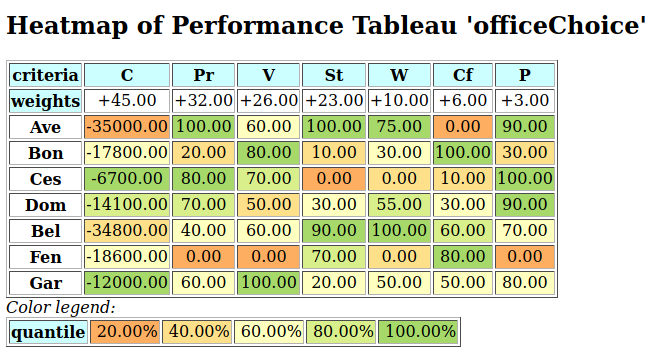
\includegraphics[width=0.8\hsize]{Figures/4-1-officeChoiceHeatmap.png}
\caption{Unranked heatmap of the office choice performance tableau}
\label{fig:4.1}       % Give a unique label
\end{figure}

Location \texttt{Ave} shows extreme and contradictory evaluations: highest \emph{Costs} and no \emph{Working Comfort} on the one hand, and total satisfaction with respect to \emph{Standing}, \emph{Proximity} and \emph{Parking facilities} on the other hand. Similar, but opposite, situation is given for location \texttt{Ces}: unsatisfactory \emph{Working Space}, no \emph{Standing} and no \emph{Working Comfort} on the one hand, and lowest \emph{Costs}, best \emph{Proximity} and \emph{Parking facilities} on the other hand. Contrary to these contradictory alternatives, we observe two appealing compromise alternatives: locations \texttt{Dom} and \texttt{Gar}. Finally, location \texttt{Fen} is clearly the less satisfactory alternative of all.

To help now the CEO choosing the best office location, we are going to compute pairwise outranking situations on the set of potential decision alternatives (see \citealp{BIS-2013}).

\section{Computing the outranking digraph}
\label{sec:4.3}

\begin{definition}[Outranking situation]\label{def:outranking}\index{outranking!situation}

\noindent For two potential decision alternatives $x$ and $y$:
\begin{itemize}[leftmargin=0.5cm,rightmargin=0.5cm]
\item ``Alternative $x$ \emph{outranks} alternative $y$'', denoted $(x \succsim y)$, is given when:
   \begin{enumerate}[nosep]
     \item A \emph{majority} of criteria significance warrants that alternative $x$ is \emph{at least as well evaluated as} alternative $y$, and
     \item \emph{No considerable} negative performance difference is observed on any criterion.      
    \end{enumerate}
\item ``Alternative $x$ \emph{does not outrank} $y$'', denoted $(x \not\succsim y)$, is given when:
   \begin{enumerate}[nosep]
    \item Only a \emph{minority} of criteria significance warrants that alternative $x$ is \emph{at least as well evaluated as} alternative $y$, and
    \item \emph{No considerable} positive performance difference is observed on any criterion. 
    \end{enumerate}
\item Otherwise, the outranking situation between alternatives $x$ and $y$ is considered to be \emph{indeterminate}.
\end{itemize}
\end{definition}

The credibility of each pairwise outranking situation, denoted $r(x \succsim y)$, is measured in a bipolar significance valuation $[-1.0, 1.0]$, where \emph{positive} terms $r(x \succsim y)\, >\, 0.0$ indicate a \emph{validated outranking}, and \emph{negative} terms $r(x \succsim y)\, <\, 0.0$ indicate an \emph{invalidated outranking}, i.e. a \emph{validated outranked} situation. The \emph{median} value $r(x \succsim y)\, = \,0.0$ represents an \emph{indeterminate} situation (see \citealp{BIS-2004a} and \citealp{BIS-2013}).   

For computing such a bipolar-valued binary outranking relation from the given performance tableau \texttt{pt}, we use the \texttt{BipolarOutrankingDigraph}\index{BipolarOutrankingDigraph@\texttt{BipolarOutrankingDigraph} class} class from the \texttt{outrankingDigraphs}\index{outrankingDigraphs@\texttt{outrankingDigraphs} module} module. The corresponding
\texttt{showHTMLRe\-lation\-Table()}\index{showHTMLRelationTable@\texttt{showHTMLRelationTable()}} method shows here the resulting bipolar-valued adjacency matrix in a system browser window (see Fig.~\vref{fig:4.2}).
\begin{lstlisting}[caption={Computing a bipolar-valued outranking digraph},label=list:4.3]
>>> from outrankingDigraphs import BipolarOutrankingDigraph
>>> bod = BipolarOutrankingDigraph(pt)
>>> bod.showHTMLRelationTable()
\end{lstlisting}
\begin{figure}[ht]
\sidecaption[t]
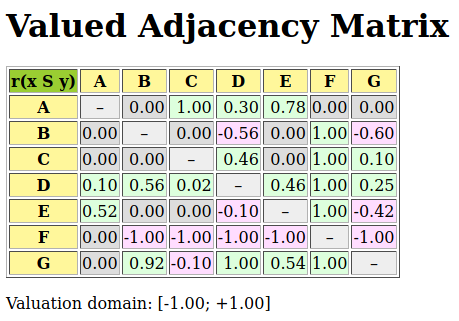
\includegraphics[width=7cm]{Figures/4-2-officeChoiceOutranking.png}
\caption[Bipolar-valued adjacency matrix]{\emph{Bipolar-valued adjacency matrix}\\ In the resulting outranking relation we may notice, on the one hand, that Alternative \texttt{D} is \emph{positively outranking} all other potential office locations. On the other hand, alternatives \texttt{A} (the most expensive) and \texttt{C} (the cheapest) are \emph{not outranked} by any other location.}
\label{fig:4.2}       % Give a unique label
\end{figure}

Alternative \texttt{D} gives a \Condorcet winner\footnote{See Chap.~\ref{sec:7} on computing the winner of an election.}, whereas alternatives \texttt{A} (the most expensive) and \texttt{C} (the cheapest) give in fact \emph{weak} \Condorcet winners.\index{computeCondorcetWinners@\texttt{computeCondorcetWinners()}}\index{computeWeakCondorcetWinners@\texttt{computeWeakCondorcetWinners()}}
\begin{lstlisting}
>>> bod.computeCondorcetWinners()
 ['D']
>>> bod.computeWeakCondorcetWinners()
 ['A', 'C', 'D']
\end{lstlisting}

From theory, we know that outranking digraphs are \emph{weakly complete}\index{weakly complete}, i.e. for all $x$ and $y$ in $X$, $r(x \succsim y)\, <\, 0.0$ implies that $r(y \succsim x)\, \geqslant \, 0.0$. And, they verify the \emph{coduality principle}\index{coduality principle}:  $r(x \not\succsim y) \; = \; r(y \succnsim x)$ \citep{BIS-2013}.\footnote{Not to be confused with the dual graph of a plane graph \texttt{g} that has a vertex for each face of \texttt{g}. Here we mean the \emph{less than} (strict converse) relation corresponding to a \emph{greater or equal} relation, or the \emph{less than or equal} relation corresponding to a (strict) \emph{better than} relation.}

\begin{definition}[Strict outranking situation]\label{def:strictOutranking}\index{outranking!strict situation}

\noindent For two potential decision alternatives $x$ and $y$, ``$x$ \emph{strictly outranks} alternative $y$'', denoted $(x \succnsim y)$, when ``$x$ \emph{outranks} alternative $y$'' ($(x \succsim y) > 0.0$) and ``$y$ \emph{does not outrank} alternative $x$'' ($(y \succsim x) < 0.0$).
\end{definition}

Following from the coduality principle, the strict outranking digraph \texttt{bodcd} is build from the outranking digraph \texttt{bod} with a codual transform\index{codual transform} (see Sect.~\ref{sec:2.6}).
\begin{lstlisting} 
>>> bodcd = ~(-bod)  # codual tranform
>>> bodcd
*------- Object instance description ------*
Instance class       : BipolarOutrankingDigraph
Instance name        : converse-dual-rel_officeChoice
Actions              : 7
Criteria             : 7
Size                 : 10
Determinateness (%)  : 72.38
Valuation domain     : [-1.00;1.00]
\end{lstlisting}


\section{Designing a best choice recommender system}
\label{sec:4.4}

Solving a best-choice problem consists traditionally in finding \emph{the} unique best decision alternative. We adopt here instead a modern recommender system’s approach which shows a non empty subset of decision alternatives which contains by construction the potential best alternative(s).

The five \emph{pragmatic principles} for computing such a \emph{best-choice recommendation} (BCR) are the following:
\begin{itemize}[leftmargin=1cm,listparindent=0em]
\item [\texttt{P1}:] \emph{Elimination for well motivated reasons}; each eliminated alternative has to be strictly outranked by at least one alternative in the BCR.
\item [\texttt{P2}:] \emph{Minimal size}; the BCR must be as limited in cardinality as possible.
\item [\texttt{P3}:] \emph{Efficient and informative}; The BCR must not contain a self-contained sub-recommendation.
\item [\texttt{P4}:] \emph{Effectively better}; the BCR must not be ambiguous in the sense that it may not be both a first choice as well as a last choice recommendation.
\item [\texttt{P5}:] \emph{Maximally determined}; the BCR is, of all potential best-choice recommendations, the most determined one in the sense of the epistemic characteristics of the bipolar-valued outranking relation.
\end{itemize}

Let $X$ be the set of potential decision alternatives. Let $Y$ be a non empty subset of $X$, called a \emph{choice} in the strict outranking digraph $G(X,r(\succnsim )$. We can now qualify a BCR $Y$ in following terms:
\begin{itemize}[leftmargin=0.5cm,listparindent=0em]
\item [-] $Y$ is called strictly \emph{outranking} (resp. \emph{outranked}) when for all not selected alternative $x$ there exists an alternative $y \in X$ retained such that $r(y \succnsim x) > 0.0$ (resp. $r(y \precsim x) > 0.0$). Such a choice verifies principle \texttt{P1}.
\item [-] $Y$ is called \emph{weakly independent} when for all $x \neq y$ in $Y$ we observe $r(x \succnsim y) \leq 0.0$. Such a choice verifies principles \texttt{P3} (\emph{internal stability}).
\item [-] $Y$ is conjointly a strictly \emph{outranking} (resp. \emph{outranked}) \textbf{and} \emph{weakly independent} choice. Such a choice is called an \emph{initial} (resp. \emph{terminal}) \emph{prekernel}\footnote{See Chap.~\ref{sec:17} on computing kernels in digraphs}. The initial prekernel now verifies principles \texttt{P1}, \texttt{P2}, \texttt{P3} and \texttt{P4}. 
\item [-] To finally verify principle \texttt{P5}, we recommend among all potential initial prekernels, a \emph{most determined} one, i.e. a strictly \emph{outranking} and \emph{weakly independent} choice supported by the highest criteria significance. And in this most determined initial prekernel we eventually retain the alternative(s) that are included with highest criteria significance\footnote{See Sect.~\ref{sec:17.6}}.
\end{itemize}

Mind that a given strict outranking digraph may not always admit prekernels. This is the case when the digraph contains chordless circuits of odd length (see Chap.~\ref{sec:17}). Luckily, our strict outranking digraph \texttt{bodcd} here does not show any chordless outranking circuits; a fact we can check with the \texttt{computeChordless\-Cir\-cuits()} method\index{computeChordlessCircuits@\texttt{computeChordlessCircuits()}} followed by the \texttt{showChordlessCircuits()} method\index{showChordlessCircuits@\texttt{showChordlessCircuits()}}\footnote{The \texttt{computeChordlessCircuits()} and \texttt{showChordlessCircuits()} methods are separate because there are various methods available for enumerating the chordless circuits in a digraph \citep{BIS-2010}.}.
\begin{lstlisting}
>>> bodcd.computeChordlessCircuits()
  []  
>>> bodcd.showChordlessCircuits()
  No circuits observed in this digraph.
\end{lstlisting}

When observing chordless odd outranking circuits, we need to break them open with the \texttt{BrokenCocsDigraph} class at their weakest link, before enumerating the prekernels. \citep{BIS-2021b}.\index{BrokenCocsDigraph@\texttt{BrokenCocsDigraph} class}

We are ready now for building a best best choice recommendation.

\section{Computing the \Rubis best choice recommendation}
\label{sec:4.5}

The \texttt{showBestChoiceRecommendation()} method\index{showBestChoiceRecommendation@\texttt{showBestChoiceRecommendation()}} computes the \Rubis best choice recommendation directly from the outranking digraph $bod$. By default this method is operating on the \emph{codual} (strict) outranking digraph where chordless odd circuits have been bropen up (see the \texttt{CoDual} and \texttt{BrokenCocs} parameters in List.~\vref{list:4.4} Line~\ref{line:4.4.2}):
\begin{lstlisting}[caption={Computing the best choice recommendation},label=list:4.4]
>>> bod.showBestChoiceRecommendation(\
...              CoDual=True, BrokenCocs=True # default settings\ §\label{line:4.4.2}§
...              ChoiceVector = True)   §\label{line:4.4.3}§
  * --- First and last choice recommendation(s) ---*
    (in decreasing order of determinateness)   
    Credibility domain: [-1.00,1.00]
    === >> potential first choice(s)
    * choice              : ['A', 'C', 'D'] §\label{line:4.4.8}§
      independence        : 0.00
      dominance           : 0.10
      absorbency          : 0.00
      covering (%)        : 41.67
      determinateness (%) : 50.59
      - characteristic vector = {
        'D': +0.02, 'G': 0.00, 'C': 0.00, 'A': 0.00, §\label{line:4.4.15}§
        'F': -0.02, 'E': -0.02, 'B': -0.02, } §\label{line:4.4.16}§
    === >> potential last choice(s) 
    * choice              : ['A', 'F'] §\label{line:4.4.18}§
      independence        : 0.00
      dominance           : -0.52
      absorbency          : 1.00
      covered (%)         : 50.00
      determinateness (%) : 50.00
      - characteristic vector = {
        'G': 0.00, 'F': 0.00, 'E': 0.00, 'D': 0.00, §\label{line:4.4.25}§
        'C': 0.00, 'B': 0.00, 'A': 0.00, }          §\label{line:4.4.26}§
\end{lstlisting}				  

It is interesting to notice in Line~\ref{line:4.4.8} above that the \Rubis \emph{first choice recommendation} consists actually in the previously mentioned set of weak \Condorcet winners\index{Condorcet@\Condorcet!winner}: \texttt{A}, \texttt{C} and \texttt{D} (see Fig.~\vref{fig:4.2}). In the corresponding prekernel characteristic vector (see Lines~\ref{line:4.4.3},~\ref{line:4.4.15} and Sect.~\ref{sec:17.6}), representing the bipolar credibility degree with which each alternative may indeed be included in, or excluded from this recommendation, we find that alternative \texttt{D} is the only positively validated one, whereas both extreme alternatives --\texttt{A} (the most expensive) and \texttt{C} (the cheapest)-- stay in an indeterminate situation (see \citealp{BIS-2006a,BIS-2006b}). They may \emph{be or not be} potential best choices. Notice furthermore that compromise alternative \texttt{G}, while not actually being included in this strictly outranking prekernel, shows as well an indeterminate situation with respect to \emph{being or not being} recommended as potential best choice. Alternatives \texttt{B}, \texttt{E} and \texttt{F} are all negatively included, i.e. positively excluded, from this best choice recommendation (see Line~\ref{line:4.4.16}).

To inspect why alternative \texttt{D} is the only positive best choice recommendation, we shall compare now the evaluations of alternatives \texttt{D} and \texttt{G} in a pairwise perspective\index{showPairwiseComparison@\texttt{showPairwiseComparison()}}.
\begin{lstlisting}[caption={Inspecting pairwise comparison between alternatives \texttt{G} and \texttt{D}},label=list:4.5,basicstyle=\ttfamily\scriptsize]
>>> bod.showPairwiseComparison('G','D')
 *------------  pairwise comparison ----*
  Comparing actions : ('G', 'D')
  crit.  wght.    g(x)      g(y)    diff.  |   ind.    pref.  concord. 
  ====================================================================
   Costs 45.00 -12000.00 -14100.00 +2100.00 | 1000.00 2500.00  +45.00  
   Comf.  6.00     50.00     30.00   +20.00 |   10.00   20.00   +6.00 
   Park.  3.00     80.00     90.00   -10.00 |   10.00   20.00   +3.00 
   Prox. 32.00     60.00     70.00   -10.00 |   10.00   20.00  +32.00 
   Stdg. 23.00     20.00     30.00   -10.00 |   10.00   20.00  +23.00 
   Visi. 26.00    100.00     50.00   +50.00 |   10.00   20.00  +26.00 
   Spac. 10.00     50.00     55.00    -5.00 |   10.00   20.00  +10.00
   =====================================================================
    Valuation in range: -145.00 to +145.00; global concordance: +145.00
\end{lstlisting}

In Listing~\vref{list:4.5}, we notice that, with the given preference discrimination thresholds, alternative \texttt{G} is actually \emph{certainly at least as well evaluated as} alternative \texttt{D}:  $r(G \succsim D)\, = \, +145/145\, =\, +1.0$.

Yet, we must as well acknowledge in Listing~\vref{list:4.6}, that the cheapest alternative \texttt{C} is in fact \emph{strictly outranking} alternative \texttt{G}:  $r(C \succsim G)\, =\, +15/145\, >\, 0.0$, and $r(G \succsim C)\, =\, -15/145 \,<\, 0.0$.
\begin{lstlisting}[caption={Inspecting pairwise comparison between alternatives \texttt{C} and \texttt{G}},label=list:4.6,basicstyle=\ttfamily\scriptsize]
>>> bod.showPairwiseComparison('C','G')
 *------------  pairwise comparison ----*
  Comparing actions : (C,G)/(G,C)
  crit. wght.   g(x)     g(y)      diff.  |   ind.   pref.       (C,G)/(G,C)
   ==========================================================================
   'C'   45.00 -6700.00 -12000.00 +5300.00 | 1000.00 2500.00    +45.00/-45.00 
   'Cf'   6.00    10.00     50.00   -40.00 |   10.00   20.00     -6.00/ +6.00 
   'P'    3.00   100.00     80.00   +20.00 |   10.00   20.00     +3.00/ -3.00 
   'Pr'  32.00    80.00     60.00   +20.00 |   10.00   20.00    +32.00/-32.00 
   'St'  23.00     0.00     20.00   -20.00 |   10.00   20.00    -23.00/+23.00 
   'V'   26.00    70.00    100.00   -30.00 |   10.00   20.00    -26.00/+26.00 
   'W'   10.00     0.00     50.00   -50.00 |   10.00   20.00    -10.00/+10.00
                                                               --------------
    Valuation in range: -145 to +145;      r(C >= G)/r(G >= c): +15.00/-15.00
\end{lstlisting}
\begin{figure}[ht]
\sidecaption[t]
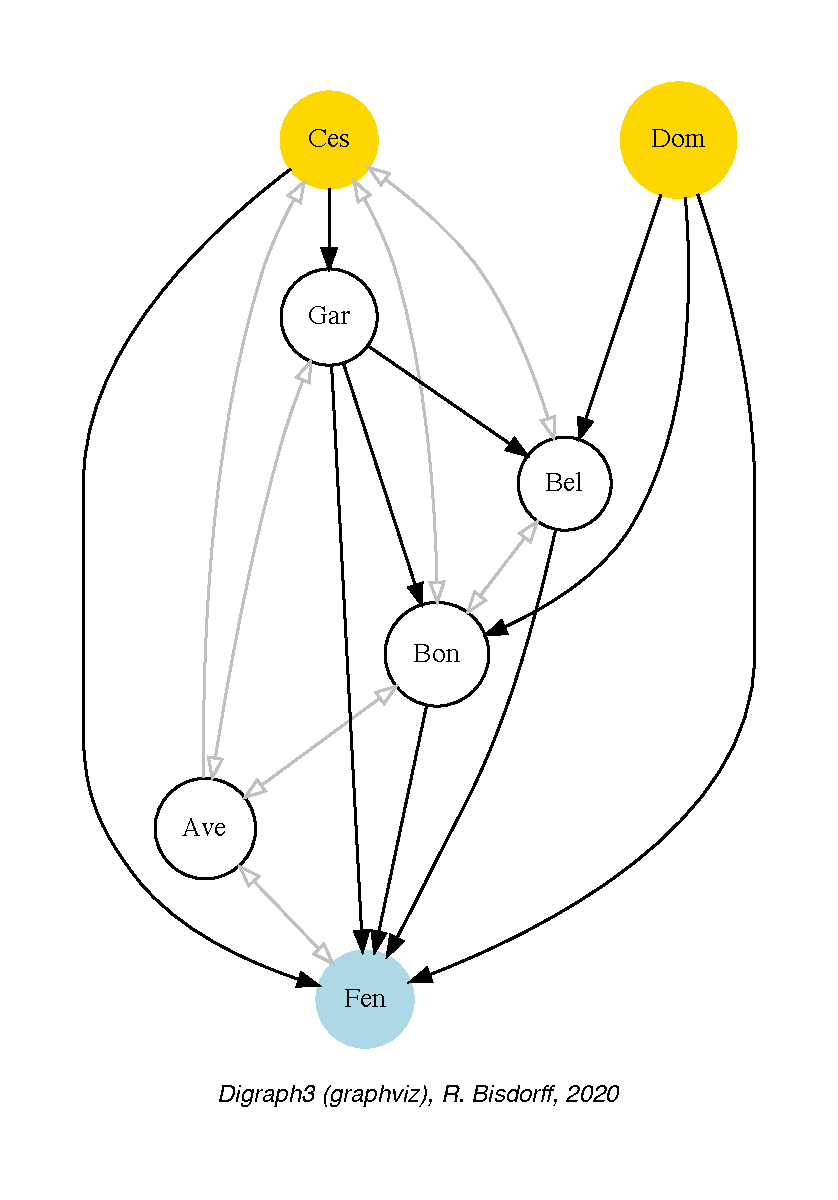
\includegraphics[width=6cm]{Figures/4-3-bestOfficeChoice.pdf}
\caption[Best office choice recommendation from strict outranking digraph]{\emph{Best office choice recommendation from strict outranking digraph}\\ Notice that location \texttt{A} (\emph{Ave}) (the most expensive) is appearing \emph{incomparable} to all the other alternatives.}
\label{fig:4.3}       % Give a unique label
\end{figure}

Let us finally notice in Listing~\vref{list:4.4} Line~\ref{line:4.4.18} that both alternatives \texttt{A} and \texttt{F} are reported as potential last choice recommendation. Yet, this last choice recommendation appears to be globally indeterminate (Lines~\ref{line:4.4.25}--\ref{line:4.4.26}). This confirms the \emph{incomparability} status of alternative \texttt{A} (see Fig.~\vref{fig:4.3}).
\begin{lstlisting}
>>> bodcd.exportGraphViz(fileName='bestOfficeChoice',\
...                    firstChoice=['C','D'],\
...                    lastChoice=['F'])
  *---- exporting a dot file for GraphViz tools ---------*
   Exporting to bestOfficeChoice.dot
   dot -Grankdir=BT -Tpng bestOfficeChoice.dot \
                    -o bestOfficeChoice.png
\end{lstlisting}

\section{Weakly ordering the outranking digraph}
\label{sec:4.6}

To get a global insight in the overall strict outranking situations, we may use the \texttt{RankingByChoosingDigraph}\index{RankingByChoosingDigraph@\texttt{RankingByChoosingDigraph} class} class imported from the \texttt{transitive\-Digraphs}\index{transitiveDigraphs@\texttt{transitiveDigraphs} module} module for computing a \emph{ranking-by-choosing} result from the codual, i.e. the strict outranking digraph instance \texttt{bodcd} (see above). If the computing node supports multiple processor cores, \emph{first} and \emph{last} choosing iterations may be run in parallel (see Line~\ref{line:4.7.4} in List.~\vref{list:4.7}).
\begin{lstlisting}[caption={Ranking-by-choosing the outranking digraph},label=list:4.7]
>>> from transitiveDigraphs import\
...                  RankingByChoosingDigraph
>>> rbc = RankingByChoosingDigraph(bodcd)
 Threading ... # multiprocessing if 2 cores are available §\label{line:4.7.4}§
 Exiting computing threads
>>> rbc.showRankingByChoosing()
 Ranking by Choosing and Rejecting
    1st ranked ['D']
       2nd ranked ['C', 'G']
       2nd last ranked ['B', 'C', 'E']
    1st last ranked ['A', 'F']
>>> rbc.exportGraphViz('officeChoiceRanking')
 *---- exporting a dot file for GraphViz tools ---------*
  Exporting to officeChoiceRanking.dot
  dot -Grankdir=TB -Tpng officeChoiceRanking.dot\
                   -o officeChoiceRanking.png
\end{lstlisting}
\begin{figure}[ht]
\sidecaption[t]
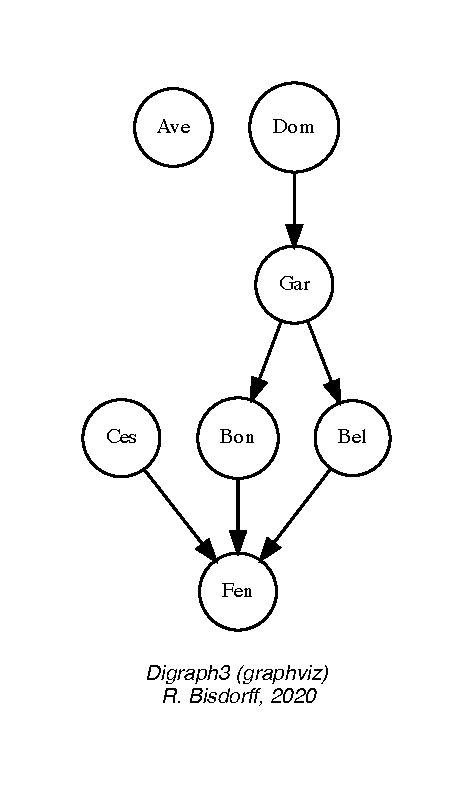
\includegraphics[width=5cm]{Figures/4-4-officeChoiceRanking.pdf}
\caption[Ranking-by-choosing the potential office locations]{\emph{Ranking-by-choosing the potentail office locations}\\ In this \emph{ranking-by-choosing} method, where we operate the \emph{epistemic fusion} of iterated (strict) first and last choices, compromise alternative \texttt{Dom} is now ranked before compromise alternative \texttt{Gar}. The overall partial ordering result shows again the important fact that the most expensive location \texttt{Ave}, and the cheapest location \texttt{Ces}, due to their contradictory performances, appear both \emph{incomparable} with most of the other alternatives.} 
\label{fig:4.4}       % Give a unique label
\end{figure}

The best choice recommendation hence depends on the very importance the CEO is attaching to each of his decision objectives. In the given setting here, where he considers that \emph{maximising the future turnover} is the most important objective followed by \emph{minimising the Costs} and, less important, \emph{maximising the working conditions}, location \texttt{D} represents actually the \emph{best compromise}. However, if \emph{Costs} do not play much a role, it would be perhaps better to decide to move to the most advantageous location \texttt{A}; or if, on the contrary, \emph{Costs} do matter a lot, moving to the cheapest alternative \texttt{C} could definitely represent a more convincing recommendation. 

It might be worth editing the criteria significance weights in the\\
\texttt{officeChoice.py} data file in such a way that:
\begin{itemize}[topsep=2pt]
\item All three decision objectives are considered \emph{equally important}, and
\item All criteria under each objective are considered \emph{equi-significant}.
\end{itemize}

What will become the best choice recommendation under this working hypothesis?\footnote{See also the notes of Lecture 7 from the MICS Algorithmic Decision Theory course \citep{ADT-L7}.} 

%\vspace{1cm}
\vspace{\baselineskip}
In the next Chap.~\ref{sec:5} we precisely show how to edit a new performance tableau from a given template file. 

%%%%%%%%%%%%%%%%%%%%%%%%%%%%%%%%%%%%
\phantomsection
\addcontentsline{toc}{section}{Notes}
\section*{Notes}

Following a seminar presentation in 2005 at the LAMSADE\footnote{Laboratoires d'Analyse et de Modélisation de Systèmes d'Aide à la Décision, Université Paris-Dauphine, UMR 7243 CNRS}, where the author promoted the use of kernels of the outranking digraph as suitable candidates for delivering best choice recommendations \citep{BIS-2005}, a critical discussion started about the methodological requirement for a convincing best choice recommendation to be internally stable (pragmatic principle \texttt{P3}). \emph{Denis Bouyssou}\index{Bouyssou@\emph{D. Bouyssou}} illustrated his doubts with the potential outranking digraph shown in Fig.~\vref{fig:4.5}.
\begin{figure}[ht]
\sidecaption[t]
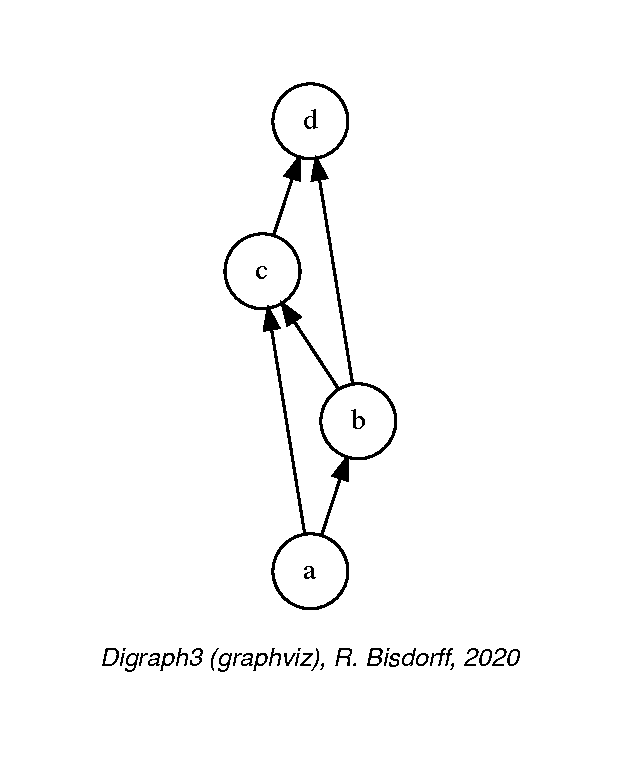
\includegraphics[width=6cm]{Figures/4-5-bouyssou11Oct05crisp.pdf}
\caption[The internal stability of a best choice recommendation in question]{\emph{The internal stability of a best choice recommendation in question}\\ The only kernel of this digraph is the pair $\{\mathtt{a},\mathtt{d}\}$; yet, it is an ambiguous recommendation, as $\{\mathtt{a},\mathtt{d}\}$ is conjointly an outranking and outranked choice. If the instability of the best choice recommendation is, however, not considered a problem then the choice $\{\mathtt{a},\mathtt{b}\}$ shows the most convincing strict outranking quality and could be considered in priority for recommendation as potential best choice candidates.}
\label{fig:4.5}       % Give a unique label
\end{figure}

His commentary was the following: Adding alternative \texttt{d} to the set of potential best choice candidates is not convincing as there exists in the given digraph the node \texttt{b}, which is better evaluated than \texttt{d}. The argument that the incomparability between \texttt{a} and \texttt{d} should favour \texttt{d} as potential best choice is interesting but another hypothesis could be that \texttt{b} perhaps outranks \texttt{a}. In this latter case, it seams clear that the actual best choice recommendation should be reduced to node \texttt{b}, unless one disposes of other information, like a performance tableau and/or the actual computation method of the outranking situations. In any case, one has to be very clear about the available information when judging a best choice procedure.

It became thereafter obvious for us all that both the lack of a specific performance tableau as well as the lack of a precisely defined algorithm for computing valid outranking situations do not allow to judge if a given digraph does indeed model a potential outranking relation. In our present bipolar-valued epistemic approach, a valid outranking digraph instance, following from a given performance tableau and the disjunctive epistemic fusion construction of the outranking relation (see Chap.~\ref{sec:3}), will necessarily verify the weak completeness condition and the coduality principle. As a consequence, incomparability situations are now modelled by epistemic indeterminateness not by the actual absence of a reciprocal outranking relation.

The digraph put forward by \emph{D. Bouyssou} in the October 2005 discussion is not weakly complete --node \texttt{a} is not outranking node \texttt{d} and vice versa-- and does hence not represent, in our present sense, a valid outranking digraph instance. Yet, it may be a partial tournament and as such it could be a strict outranking digraph, i.e. the asymmetric part --the codual-- of a valid outranking digraph. In this case, nodes \texttt{a} and \texttt{d} --the kernel of the strict outranking digraph-- would actually for sure outrank each other and, hence, represent both indifferently the natural best choice recommendation. However, in this not strict codual digraph, node \texttt{a} becomes also the unique \Condorcet winner --outranking for sure all other nodes-- and gives hence the evident unique best choice recommendation.

Only after 2013, when the weak completeness and the coduality properties of the outranking digraph were discovered, became it obvious that the initial prekernels of the strict outranking digraph, coupled with the solution of the corresponding kernel equation system, were in fact delivering the most convincing best choice recommendations (see Chap.~\ref{sec:17}, Sect.~\ref{sec:20.4} and \citealp{BIS-2013}). It stays an interesting open mathematical problem to show (or not) that both necessary conditions: --weak completeness and coduality-- are also sufficient for qualifying any bipolar-valued digraph as potential instance of an outranking digraph.


%%%%%%% The chapter bibliography
%\normallatexbib
%\clearpage
%\phantomsection
%\addcontentsline{toc}{section}{Chapter Bibliography}
\input{Bibliographies/04-chapterBestChoice.bbl}
%\bibliographystyle{spbasic}
%\bibliography{03-backMatters/reference}

%\bibliographystyle{spbasic}
%\bibliography{03-backMatters/reference}

%\bibliographystyle{spbasic}
%\bibliography{03-backMatters/reference}

\bibliographystyle{spbasic}
\bibliography{03-backMatters/reference}
